\chapter{使用机器人}

% 场景为操作和使用机器人的基本功能模块,编写一个新场景即可开始操作机器人。

在讲述如何创建和编写一个场景之前,我们先了解下乐白机器人的场景编辑器以及如何进行拖动示教\footnote{拖动示教:即让机器人根据人手的拖拽来带动机器人,同时在正确设置末端工具质量和质心情况下,机器人可以达到一个自我平衡的运行状态。}操作。

\vspace*{-0.8em}

\section{场景编辑器}

您可以在场景编辑器内对机器人进行编程,即编写场景。
% \vspace*{-0.2em}
\subsection{编辑器类型}

场景提供两种编辑器:
% 乐白机器人的场景支持使用如下两种编辑器进行编程:
\begin{itemize}[leftmargin=6.5em]
	\item [时间轴编辑器]

	可视化、低门槛且无需理解任何逻辑关系的场景编辑器。适合初学者,只需要在时间轴编辑器中根据需要添加相应的动作块\footnote{场景的时间轴编辑器中,每个可操作的独立元素称作一个动作块(Block),若干个动作块的集合可以打包成为动作包。},即可让机器人运动起来(如\prettyref{fig:时间轴编辑器})。

	\item [代码编辑器]

	基于Lua语言,支持复杂的逻辑操作的场景编辑器。适合具备一定编程基础和逻辑思维的用户,通过编写相应的代码,即可让机器人运动起来(如\prettyref{fig:代码编辑器})。

\end{itemize}

	\begin{figure}[htb]
		\centering
		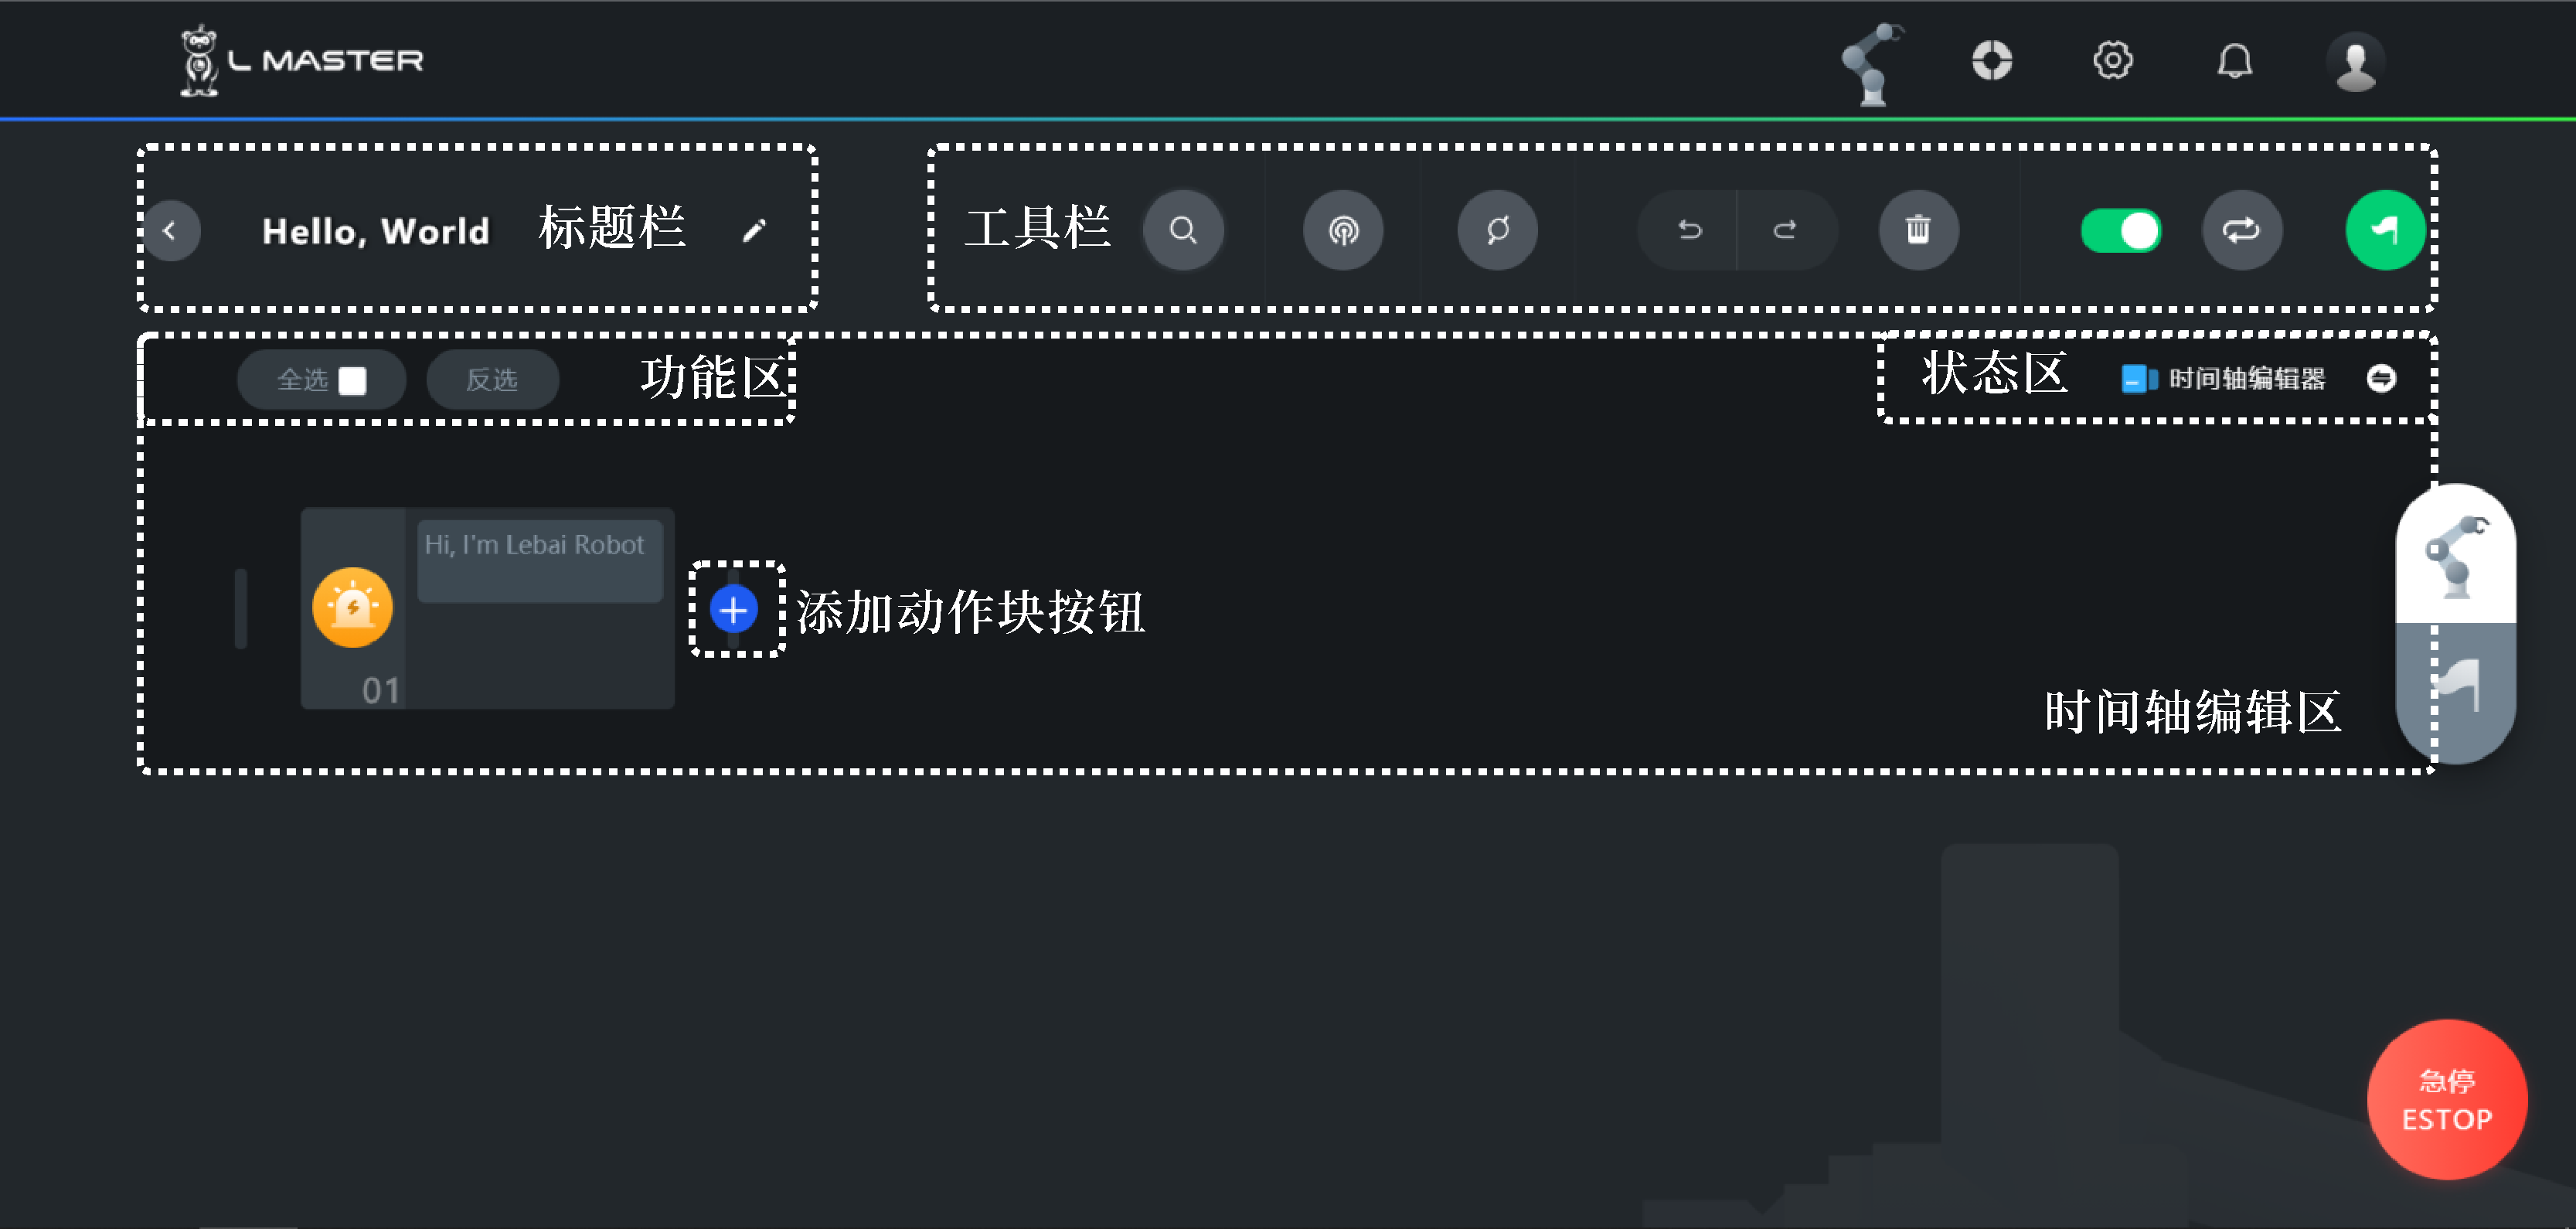
\includegraphics[width=\textwidth]{shots/timeline_editor.pdf}
		\caption{时间轴编辑器
		% \protect\footnotemark
		}
		\label{fig:时间轴编辑器}

		\vfill

		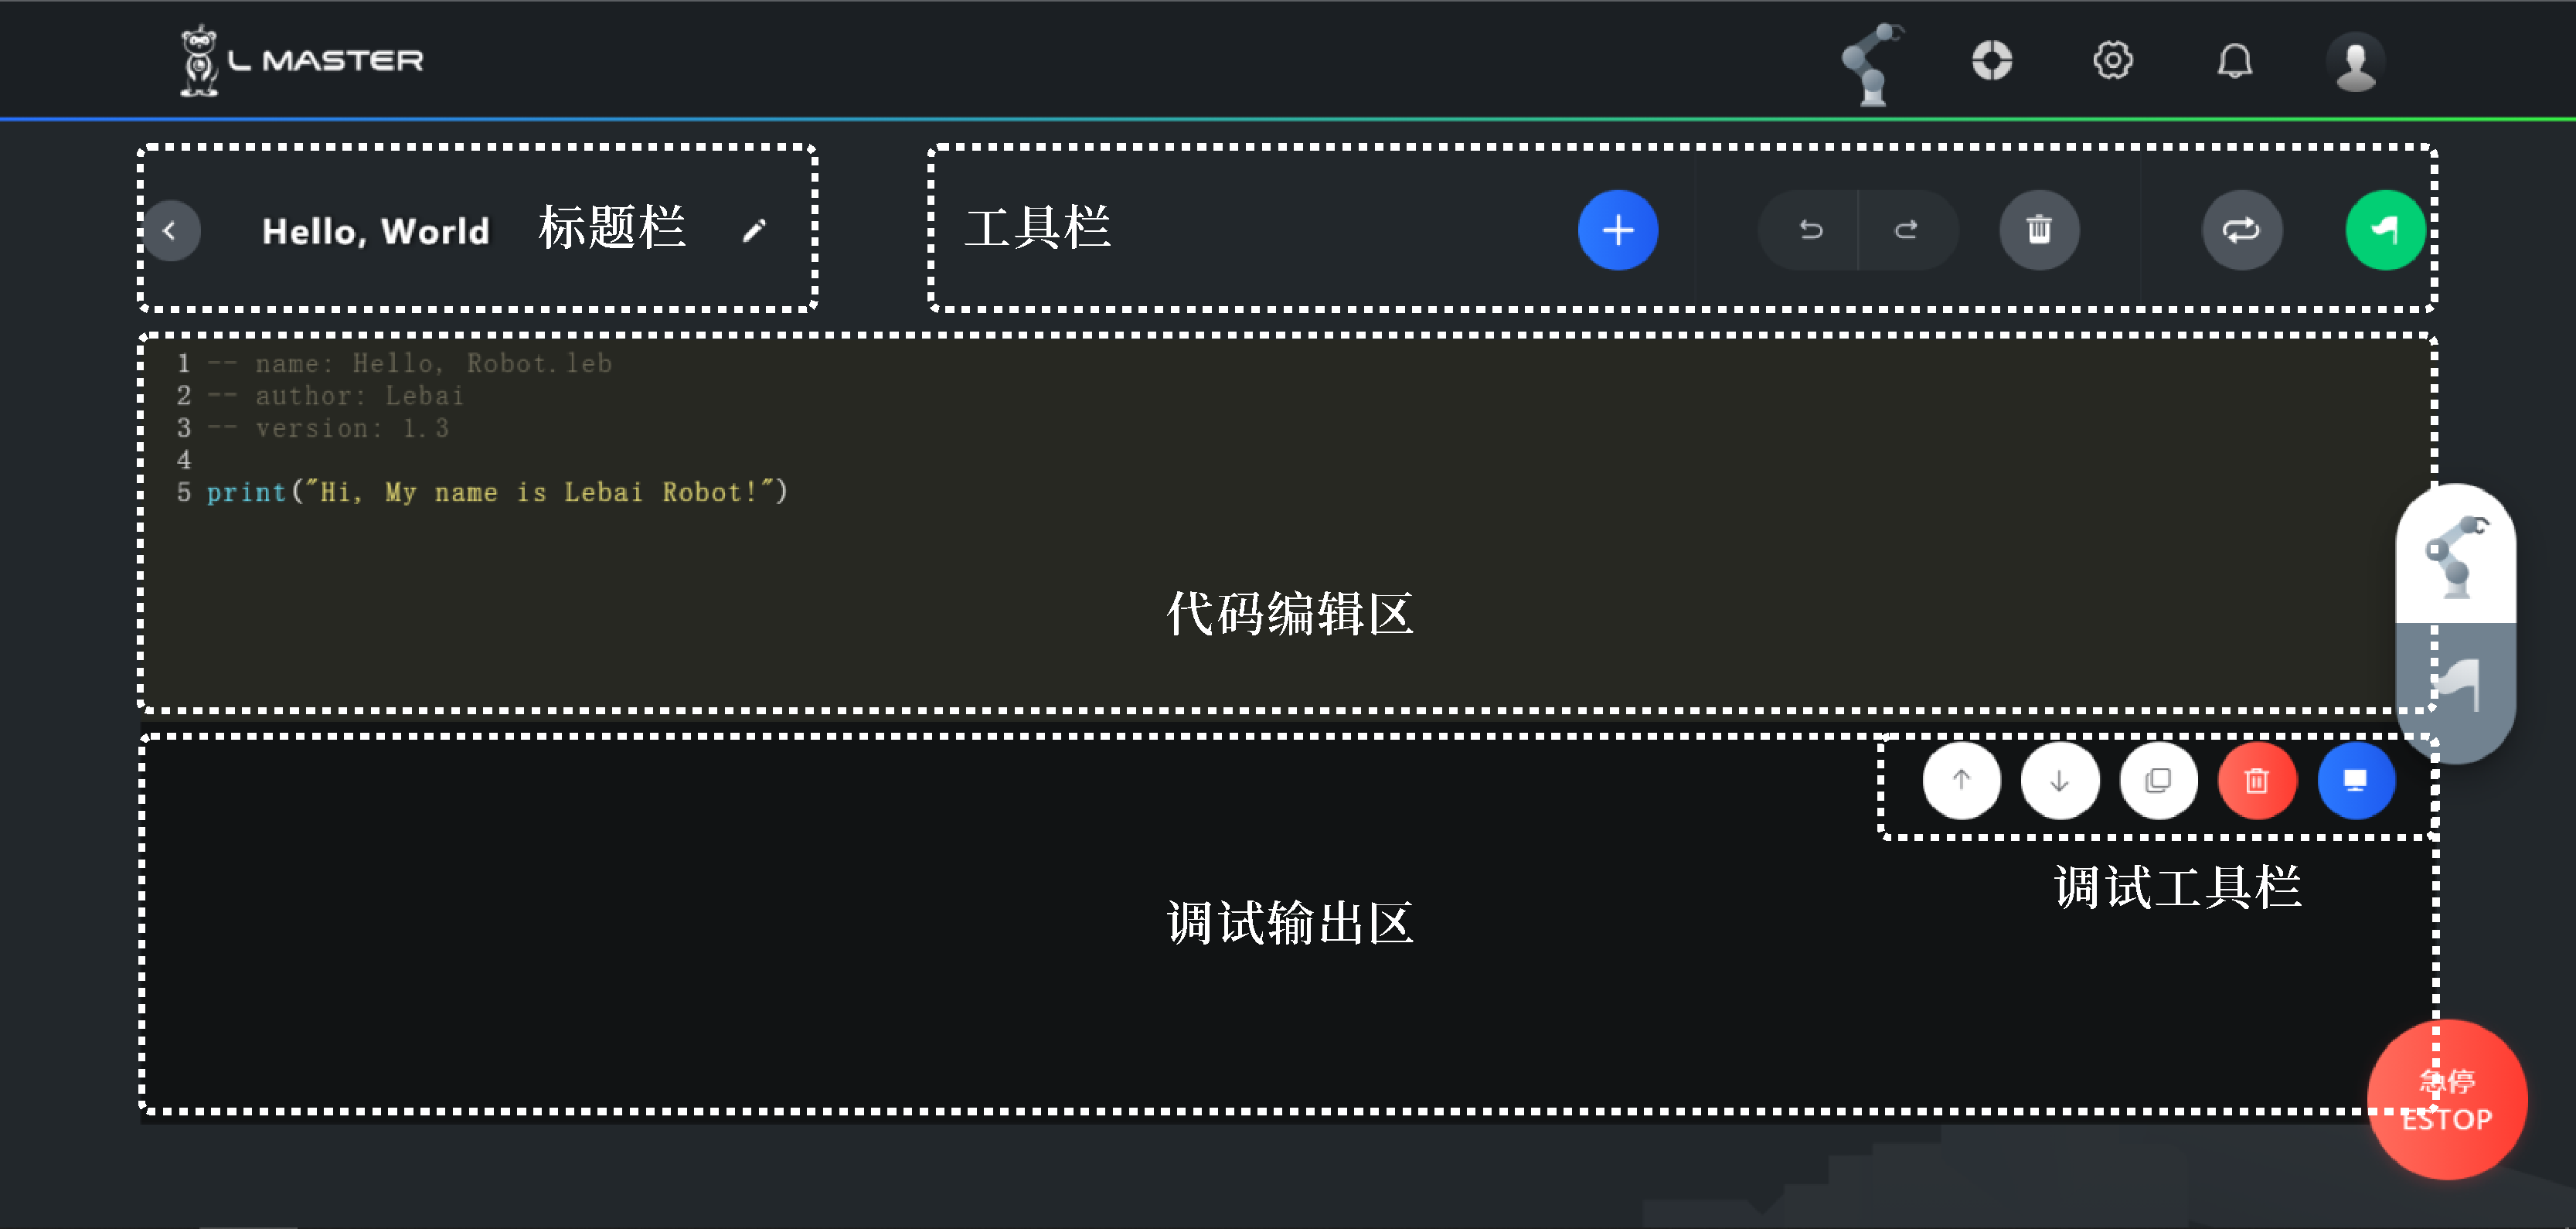
\includegraphics[width=\textwidth]{shots/code_editor.pdf}
		\caption{代码编辑器}
		\label{fig:代码编辑器}
	\end{figure}
			% \footnotetext{时间轴编辑器:以时间先后顺序展现机器人的顺序执行的动作列表,上海乐白机器人自主设计和研发的且拥有自主知识产权的专为机器人控制系统设计和研发的机器人场景编辑器。}

\clearpage

\subsection{切换编辑器类型}

代码编辑器仅在专家模式下可用,从时间轴编辑器转换到代码编辑器的步骤如下:
\begin{enumerate}
\item 进入\mnu{设置},点击\mnu{操作模式},或者点击状态区\mnu{时间轴编辑器} 右边的\colorbox{Black}{\icn{image/21.pdf}}按钮,进入操作模式选择页,选择\mnu{专家模式},点击操作模式页右上角的\btn{保存}按钮。
\item 返回之前编辑的场景。
\item 在时间轴编辑器中,鼠标移动到\mnu{时间轴编辑器}按钮上,在弹出的菜单中选择\mnu{代码编辑器}进行切换。
\end{enumerate}

\begin{figure}[H]
	\centering
	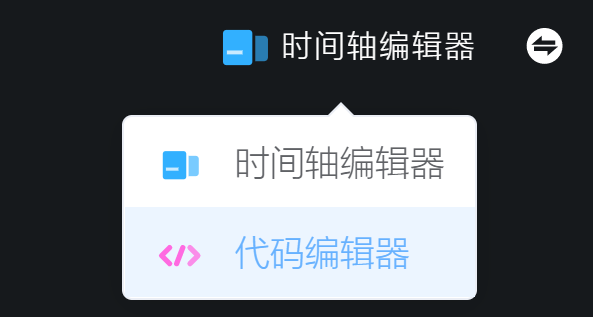
\includegraphics[height=2cm]{screen/3-3.png}
	\caption{切换编辑器类型}
	\label{fig:切换编辑器类型}
\end{figure}

\info{当某个场景的编辑器类型从时间轴编辑器切换成代码编辑器后,无法再反向转换回去。操作之前请使用 \mnu{导出} \footnote{详见\prettyref{sec:导出场景}。} 或 \mnu{复制} 功能进行备份。}

\vfill

\clearpage

% \subsection{类型图标说明}
% \begin{itemize}
% 	\item[\icn{image/43.pdf}] 在场景列表和场景编辑器页面出现此图标表示该场景为时间轴编辑器类型;
% 	\item[\icn{image/44.pdf}] 在场景列表和场景编辑器页面出现此图标表示该场景为代码编辑器类型。
% \end{itemize}

\section{拖动示教}
在讲述如何添加位置动作块之前,有必要先了解乐白机器人的拖动示教方法。拖动示教有如下两种操作方法,可任选其一:
\begin{itemize}
	\item 在\LM 点击示教图标\icn{image/36.pdf}使机器人启用示教模式,拖动机器人到达指定位置,再次点击示教图标,退出示教模式。
	\item 长按机器人末端凸按钮\footnote{详见\prettyref{sec:硬件按钮}。},使机器人启用示教模式,拖动机器人到达指定位置后,释放机器人末端凸按钮,退出示教模式。
\end{itemize}

\danger[警告]{在使用拖动示教前,请务必确保正确设置好末端设备\footnote{详见\prettyref{sec:末端设备}。}的质量与质心,不正确的设置可能导致误伤。\footnote{详见\prettyref{sec:运行安全}。}}

\danger[警告]{示教过程中注意关节角度的转动不可超出安全范围\footnote{详见\prettyref{sec:运行安全}。},否则可能导致机器人急停或其他故障。}

\vfill

\clearpage

\section{编写场景}
\subsection{创建新场景}
点击\LM 首页的\mnu{场景}按钮,进入\mnu{场景列表},点击该页面工具栏右侧的\btn[Info]{添加场景}按钮,输入场景名称,完成新场景的创建。

\begin{figure}[ht]
	\centering
	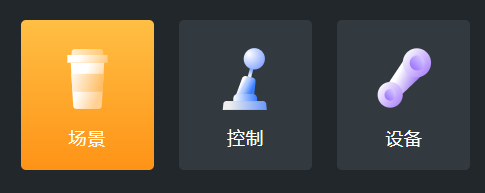
\includegraphics[height=2cm]{screen/3-4.png}
	\caption{场景入口}
	\label{fig:场景入口}
\end{figure}

\subsection{添加动作块}

时间轴编辑器支持的动作块类型有:
\begin{itemize}
\item 位置
\item 手爪
\item 等待
\item 消息提示
\item 数字I/O
\item 模拟I/O
\item 信号量
\item 负载配置
\end{itemize}

点击时间轴编辑器的添加动作块按钮\icn{image/plus.pdf},可以弹出\nameref{fig:添加动作块弹出框},如\prettyref{fig:添加动作块弹出框}所示。

\begin{figure}[ht]
	\centering
	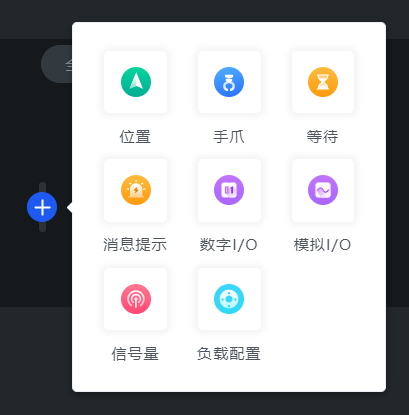
\includegraphics[width=5cm]{screen/3-5.png}
	\caption{动作块选择框}
	\label{fig:添加动作块弹出框}
\end{figure}

下面章节依次讲述不同动作块类型的使用方法。

\subsubsection{位置动作块}
位置\footnote{{\ThisBook}提到的位置是机器人位置和姿态数据的简称,本文档后续没有明确提及位置和姿态时的位置均表示机器人的位置和姿态。}控制作为机器人控制里面的核心控制模块,在时间轴编辑器中,只需要按照如下教程添加位置动作块,即可让机器人按照预定的位置动作进行相应类型的轨迹运动。
\paragraph{添加位置}
在时间轴编辑器中添加位置有如下两种操作方法,可任选其一:
\begin{itemize}
	\item 时间轴编辑器内编辑区的添加动作块按钮\icn{image/plus.pdf},选择\mnu{位置},在打开的\nameref{fig:添加位置对话框}(如\prettyref{fig:添加位置对话框}所示)中输入位置名称,点击\btn{添加}按钮,即可将机器人当前位置保存在一个新的位置动作块\footnote{动作块是时间轴编辑器里的最小可视化编辑模块,一个模块代表一种动作类型,动作类型包括:位置、I/O等。}。
	\item 双击机器人末端凸按钮,系统将机器人当前位置保存在一个新的位置动作块。
\end{itemize}

\begin{figure}[ht]
	\centering
	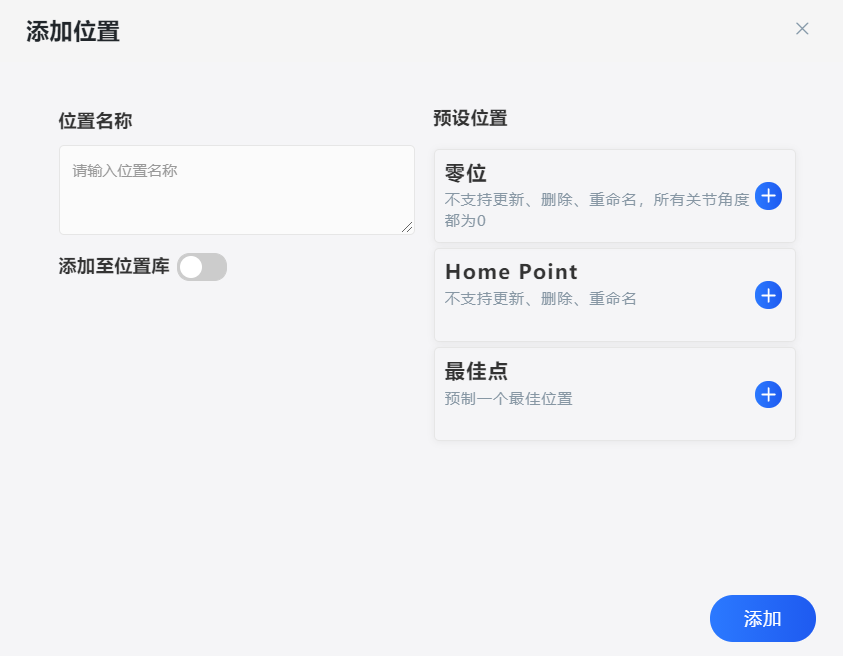
\includegraphics[height=6cm]{screen/3-6.png}
	\caption{“添加位置”对话框}
	\label{fig:添加位置对话框}
\end{figure}

通过结合拖动示教和上述添加位置动作块的方法,按照您的需求添加想要的位置动作块(可任意多个),直至场景编写完成。

\paragraph{编辑位置}
\label{sec:编辑位置}
如\prettyref{fig:位置块焦点状态},将光标放在位置块上使当前位置块处于焦点状态。

\begin{figure}[ht]
	\centering
	\includegraphics[height=3.5cm]{image/15.pdf}
	\caption{位置块焦点状态}
	\label{fig:位置块焦点状态}
\end{figure}

轨迹类型切换区的两个按钮用于切换关节空间的运动(movej)和笛卡尔空间的直线运动(movel)。
\begin{itemize}
	\item[\icn{image/ic_joint.pdf}] 表示关节空间\footnote{关节空间:以机器人每个关节角度来描述的机器人运动空间。}的运动;
	\item[\icn{image/ic_line.pdf}] 表示笛卡尔空间\footnote{笛卡尔空间:全称笛卡尔坐标系空间,即我们常用的直角坐标系空间。}的直线运动。
\end{itemize}

编辑操作按钮区从左至右的按钮依次为:

\begin{itemize}
\item [\quad] {\sffamily\bfseries 样式}:可以更换动作块背景颜色\footnote{{样式}按钮的颜色与动作块背景色保持一致,当选中动作块时会以该颜色为背景高亮该动作块。特殊地,默认样式为透明,此时动作块选中之后的高亮背景色为蓝色。样式、复制、删除按钮都是动作块操作按钮区的通用按钮。}。
\item [\icn{image/ic_adjust.pdf}] {\sffamily\bfseries 微调}:对当前位置块存储的位置数据进行微调及更新。
\item [\icn{image/ic_a_v.pdf}] {\sffamily\bfseries 速度及加速时间}:调整位置块的速度和加速时间\footnote{加速时间与加速度成反比,加速度越大,加速时间越短,反之则越长。}。
\item [\icn{image/ic_copy.pdf}] {\sffamily\bfseries 复制}:复制一个当前的动作块。
\item [\icn{image/ic_delete.pdf}] {\sffamily\bfseries 删除}:可删除当前动作块。
\end{itemize}

\paragraph{微调}
\label{sec:微调}
在编辑场景时,动作轨迹中的位置需要精准细微调整,可以对单个位置进行微调。选择微调图标,页面可自动跳转至微调页面。

% 微调页面中虚拟机器人和真实机器人底座重叠展示,其中虚拟机器人表示当前位置块存储的目标位置,真实机器人表示机器人当前位置。
当机器人当前\mnu{实际位置}与位置块存储的\mnu{目标位置}不一致时,微调页面中会出现虚拟机器人与真实机器人,其中虚拟机器人表示当前位置块存储的目标位置,真实机器人表示机器人当前的实际位置。

通过实际位置\icn{image/position.pdf}和目标位置\icn{image/saved.pdf}切换按钮进行切换,可查看目标位置与实际位置的数值。

\subparagraph{坐标空间微调}

\begin{figure}[ht]
	\centering
	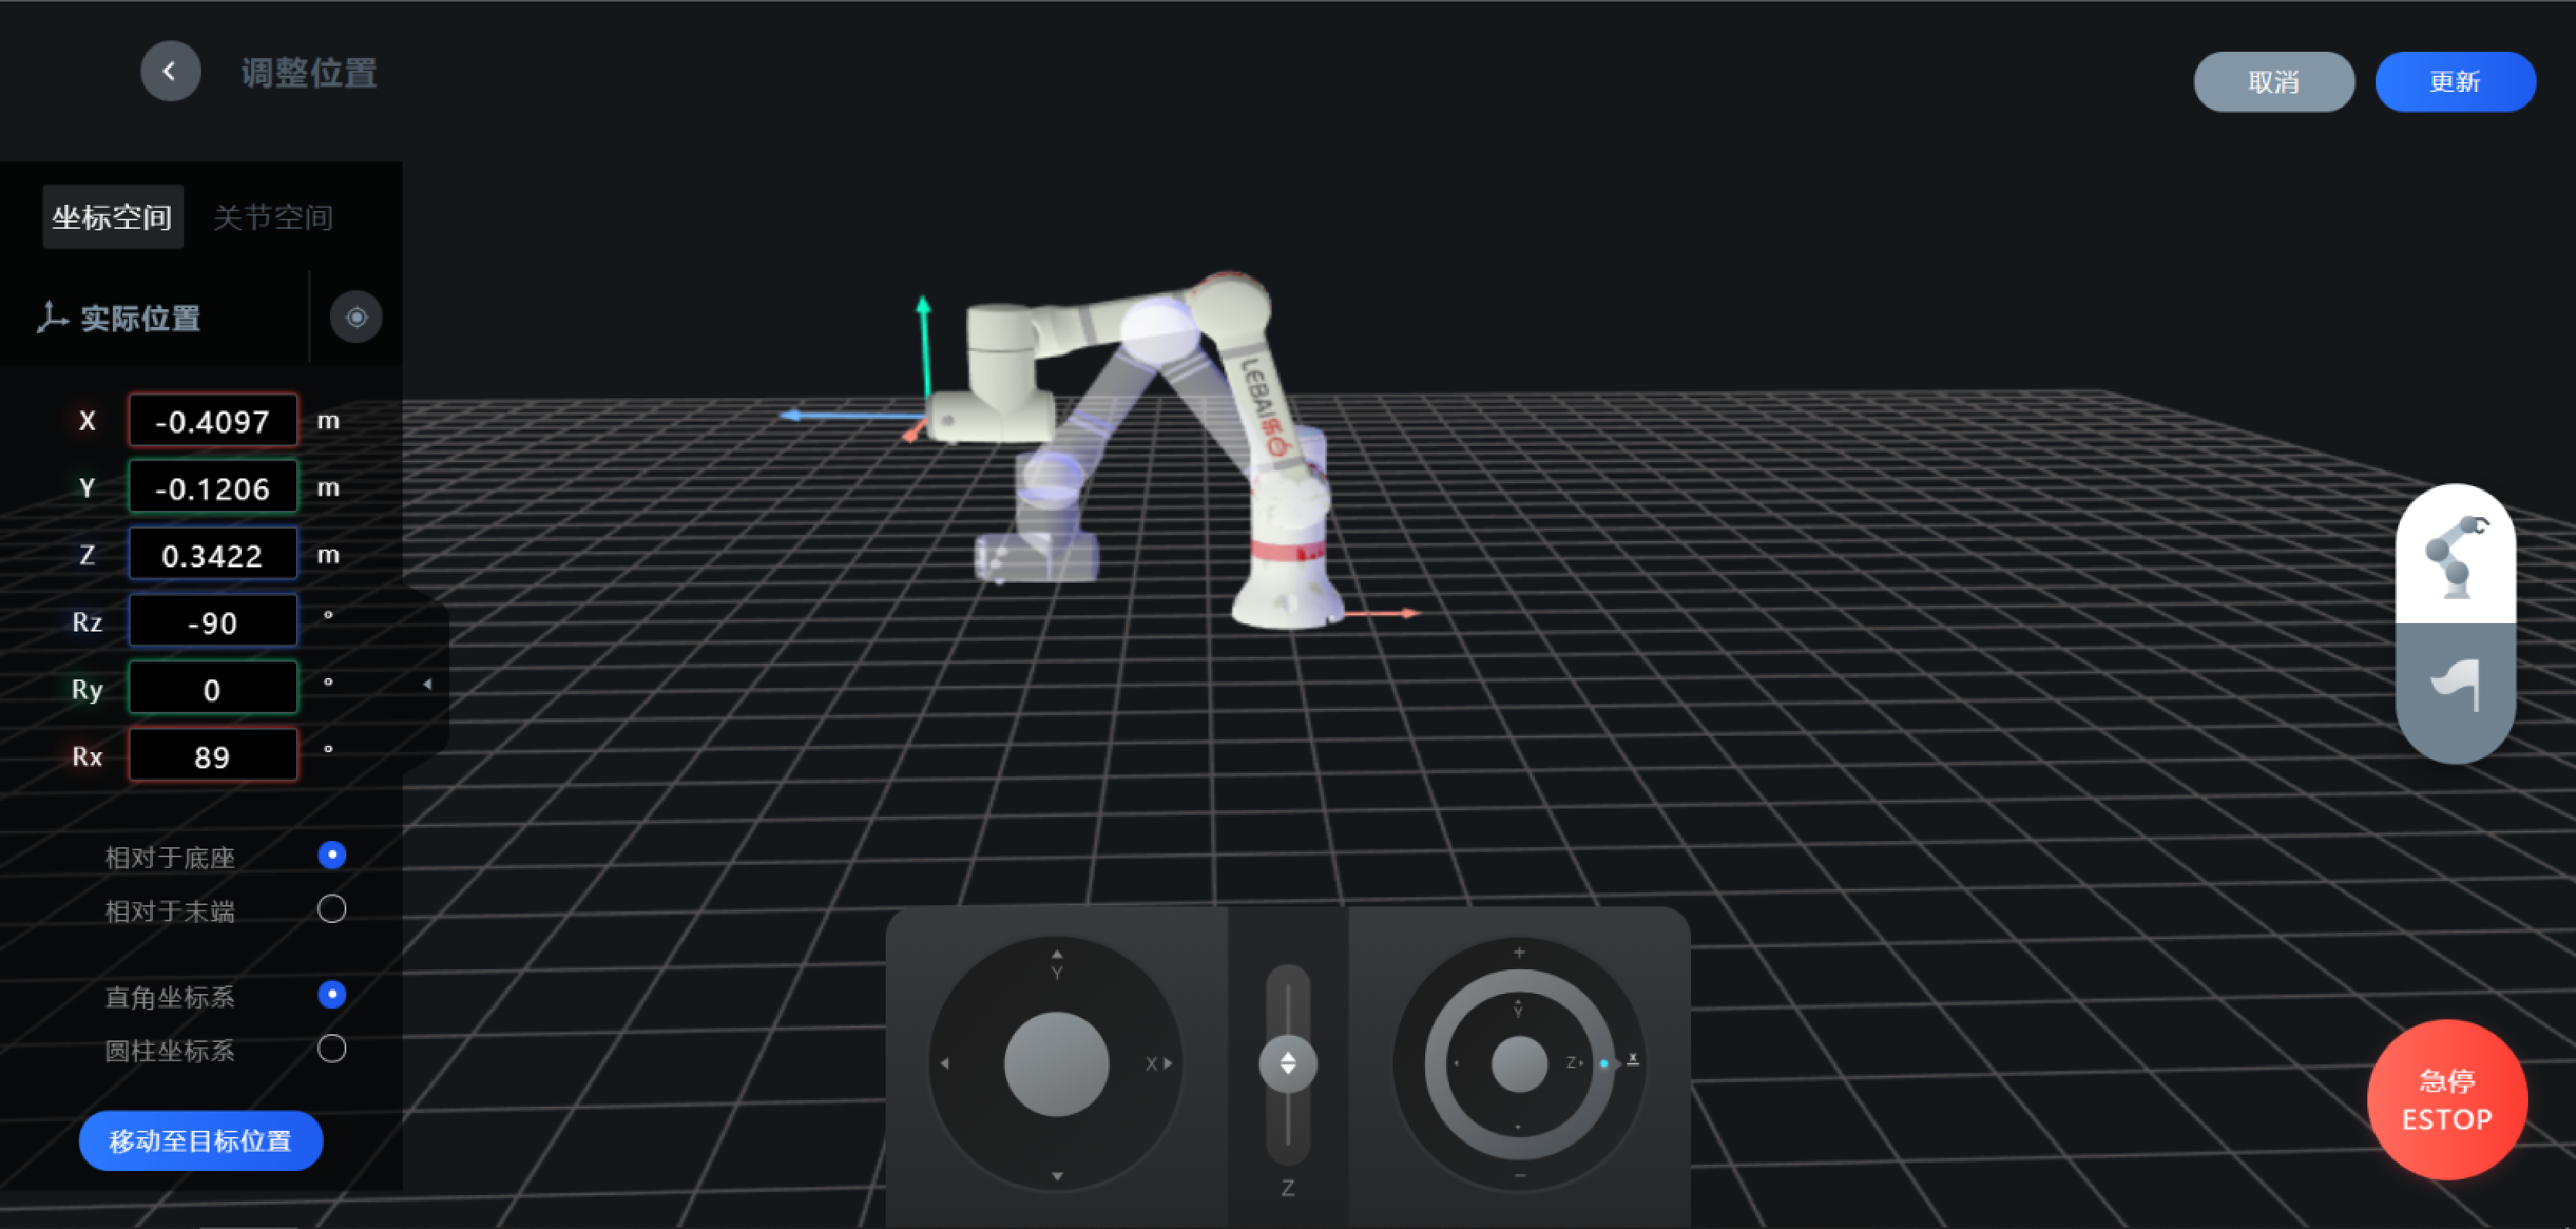
\includegraphics[width=\textwidth]{shots/fine_tuning_cartesian.pdf}
	\caption{坐标空间微调}
	\label{fig:坐标空间微调}
\end{figure}

微调时可以选择不同的坐标系表示方式:
\begin{itemize}
	\item 相对于底座时,可使用直角坐标系或圆柱坐标系。
	\item 相对于末端时,仅支持直角坐标系。
\end{itemize}

\begin{figure}[ht]
	\centering
	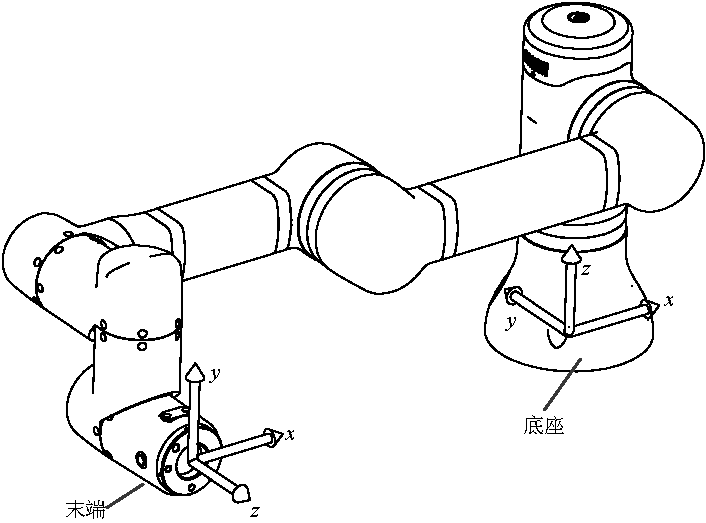
\includegraphics[height=6cm]{line_graphs/fine_tuning_coordinate.pdf}
	\caption{底座和末端坐标系}
	\label{fig:坐标空间示意图}
\end{figure}

当参考坐标系选择\mnu{相对于底座}时,表示以机器人底座平面的圆心作为世界坐标系原点。

通过选择直角坐标系为调整方式,在微调页面位置信息展示框中输入位置$(X, Y, Z)$或姿态$(R_z, R_y, R_x)$\footnote{乐白机器人在笛卡尔空间(直角坐标系空间)的姿态表示采用的是EulerZYX(欧拉ZYX)表示法,关于EulerZYX表示法可参考相关机器人基础的书籍或教程。姿态$(R_z, R_y, R_x)$也可以描述成$(\alpha, \beta, \gamma)$。}的数值,机器人会自动移动到您所需要的位置;或通过拉动屏幕下方各个方向的拉杆进行操作,当释放拉杆时,微调停止。点击\btn{更新}按钮,完成位置微调。

乐白机器人采用$Z\textrm{-}Y\textrm{-}X$欧拉角(EulerZYX)描述机器人末端的姿态,即先绕坐标系$Z$轴旋转$R_z$角,再绕旋转后的坐标系$Y$轴旋转$R_y$角,最后绕旋转两次后的坐标系$X$轴旋转$R_x$角。

选择圆柱坐标系\footnote{圆柱坐标系的$X\textrm{-}Y$平面为极坐标系。在直角坐标系的点$P(x, y, z)$表示为圆柱坐标系的$P'(\rho, \theta, z)$,其中 $\rho=\sqrt{x^2+y^2}$,$\theta=\arctan\frac{y}{x}$。},左侧调整盘会由调整$(X, Y)$变为调整$(\rho, \theta)$。

当参考坐标系选择\mnu{相对于末端}时(在不添加TCP的情况下\footnote{详见\prettyref{sec:TCP设置}。}),就是以机器人法兰盘平面的圆心作为坐标系原点,以直角坐标系为调整方式,通过在微调页面输入位置或姿态的数值或拉动屏幕下方的拉杆操作,机器人自动移动到指定位置后,点击\btn{更新},完成位置微调。

\subparagraph{关节空间微调}
点击微调页面左上方\mnu{关节空间},通过输入关节1至关节6的角度数值,机器人会自动到达指定位置;或通过拉动屏幕下方各个方向的拉杆进行操作,当释放拉杆时,微调停止,点击\btn{更新},完成位置微调。

\begin{figure}[ht]
	\centering
	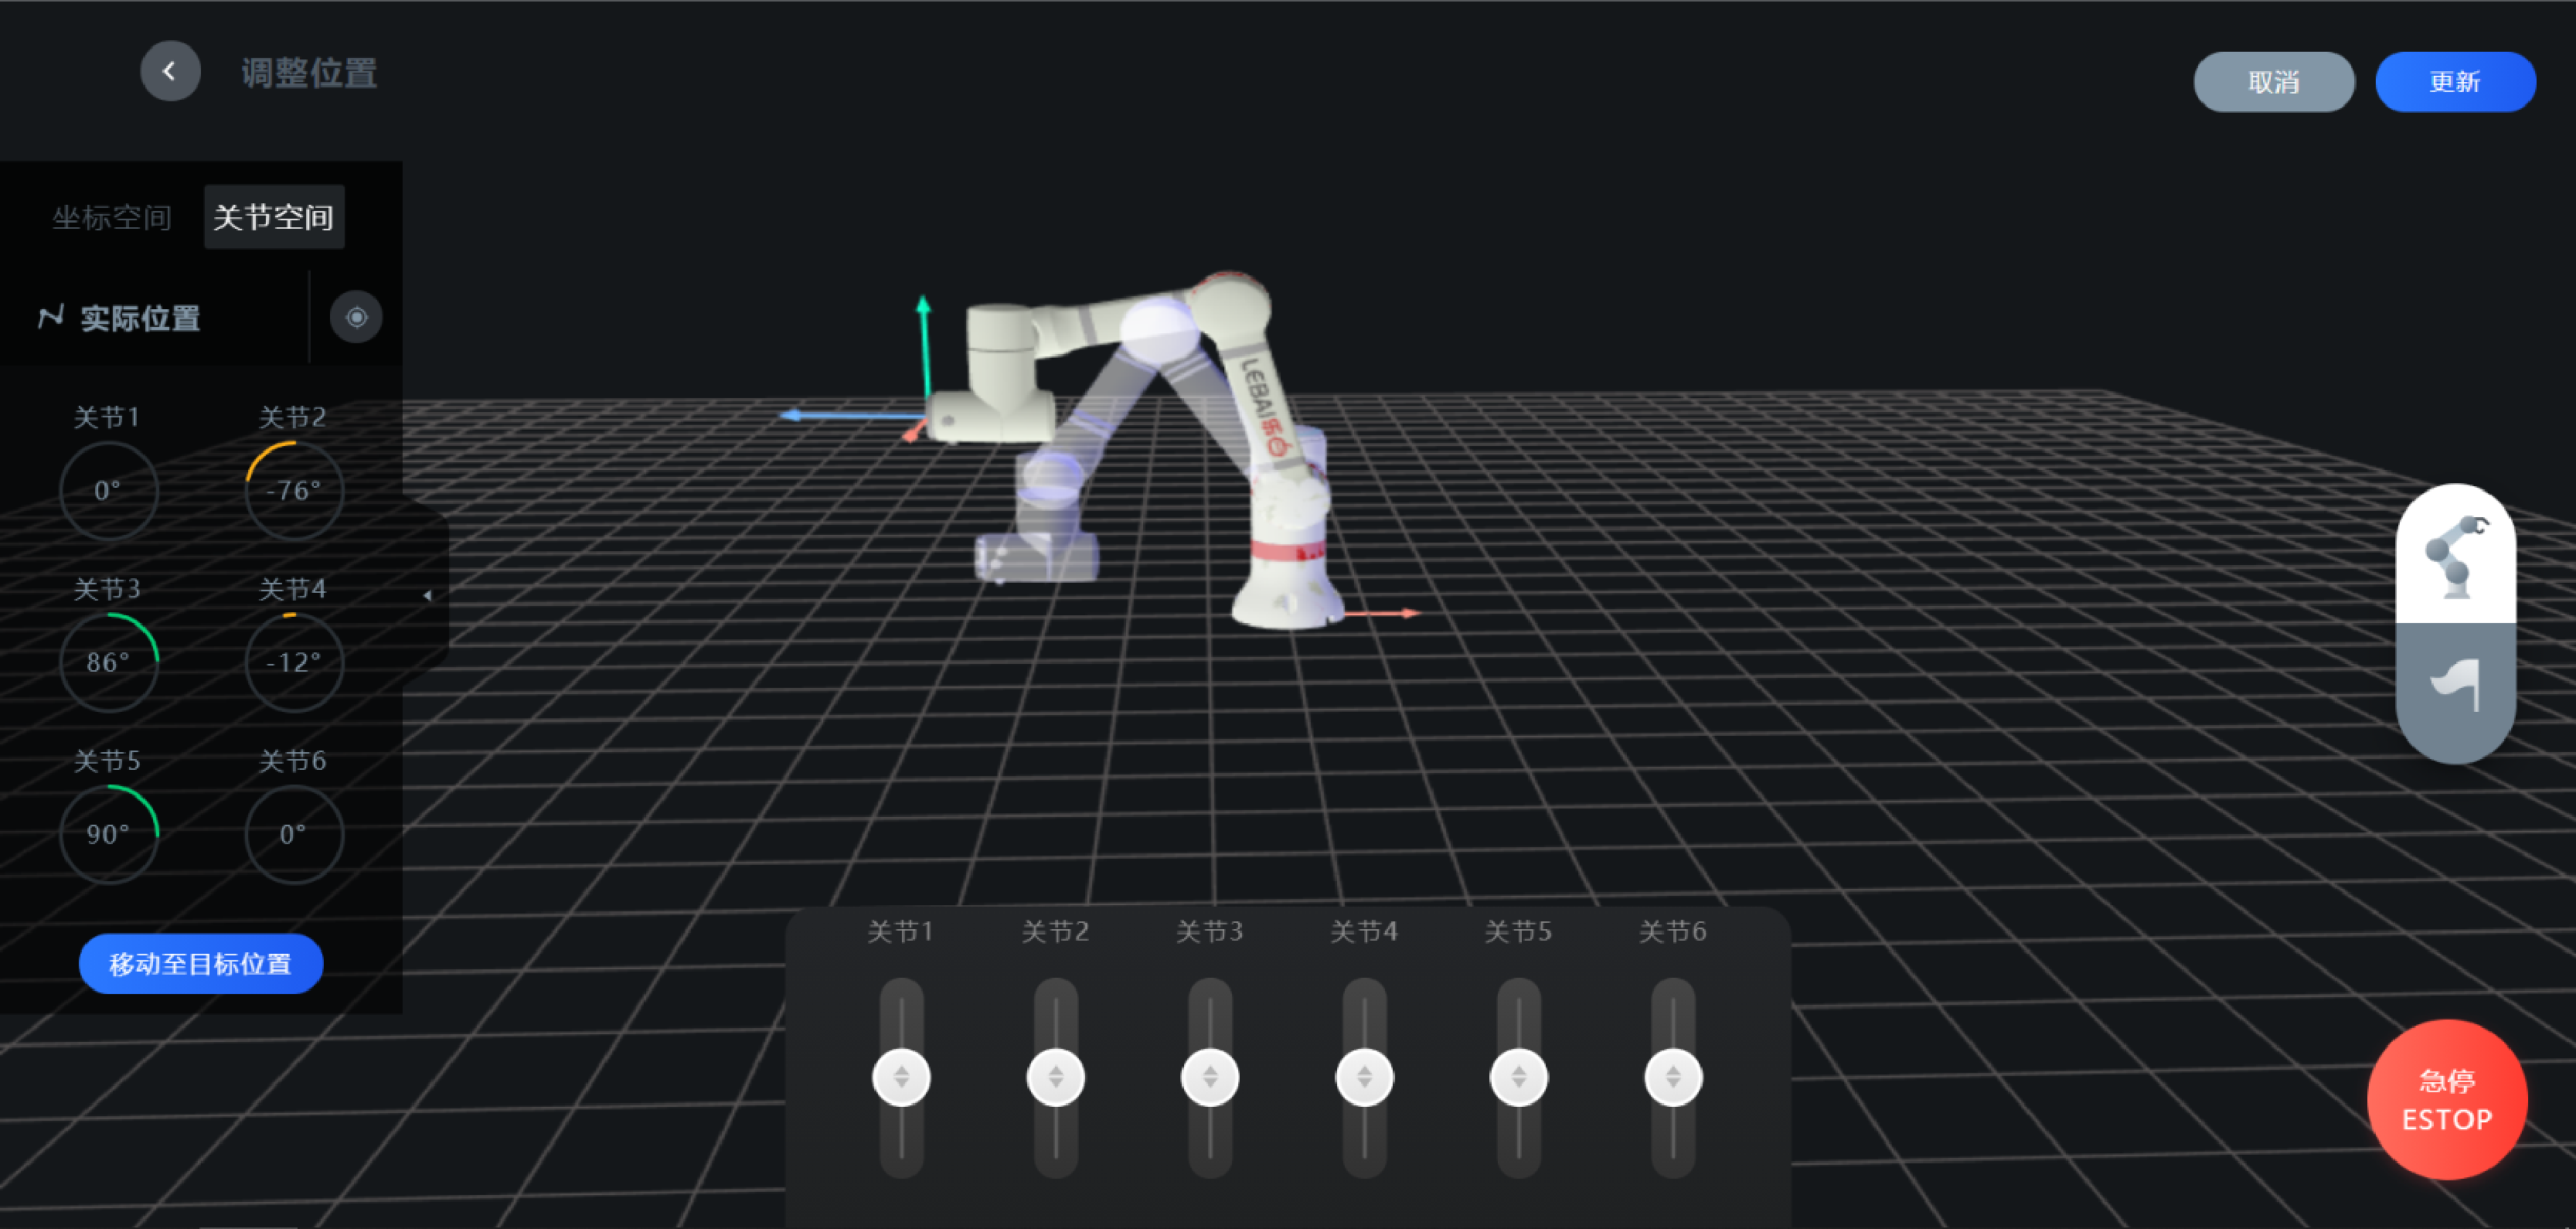
\includegraphics[width=\textwidth]{shots/fine_tuning_joint.pdf}
	\caption{关节空间微调}
	\label{fig:关节空间微调}
\end{figure}

\paragraph{速度与加速时间}
速度与加速时间是针对当前场景或单个位置块的速度$v$和加速度$a$进行修改,其中横轴对应加速时间,横轴数值越靠近原点,加速时间越短,加速度越大。纵轴对应速度,纵轴越靠近原点,速度越小。

\begin{figure}[ht]
	\centering
	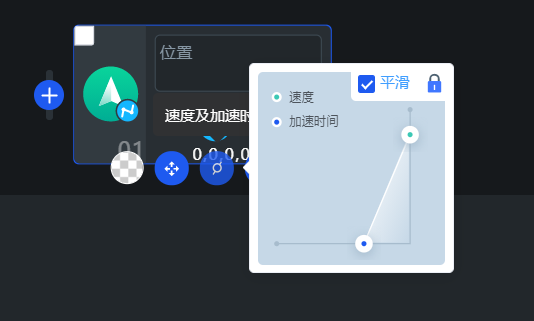
\includegraphics[height=4cm]{screen/3-11.png}
	\caption{“速度与加速时间”调整控件}
	\label{fig:速度与加速时间}
\end{figure}

速度与加速时间的调整,用户可以在场景编辑器的工具栏上全局操作\footnote{详见\prettyref{sec:速度和加速时间}。},也可以对每个位置块单独操作。

点击位置块\icn{image/ic_a_v.pdf}按钮弹出\nameref{fig:速度与加速时间},右上角的\icn{image/lock.pdf}为当前位置块与编辑器工具栏上的全局速度和加速时间信息的同步锁。当场景中添加新的位置时,该位置块的速度加速时间控件全局锁默认为锁定状态,即表示与当前场景的全局速度和加速时间保持一致;当用户拖拽调整控件的横轴或纵轴任意一个拖拽点,使速度与加速时间发生变化时,全局锁解锁,即该位置块使用自己指定的速度和加速时间,不再使用全局的速度和加速时间参数值;用户可以再次点击\icn{image/unlock.pdf}图标锁定同步锁,则该位置块又保持与全局速度与加速时间一致的参数值。

平滑功能,主要是指存在连续相邻多个位置块时,机器人控制系统自动优化出最佳路径,不停止地经过当前位置块的目标位置,使得动作连续性更好,移动的时间更短,效率更高。具体表现为当打开平滑功能之后,机器人位置间移动时,两个动作块之间不会出现明显的机器人位置间移动时的减速停止现象。

在添加完位置动作块后,如果不需要添加其他类型的动作块,则可以直接查看\prettyref{sec:运行场景}的内容。

\subsubsection{手爪动作块}

\begin{figure}[htb]
	\centering
	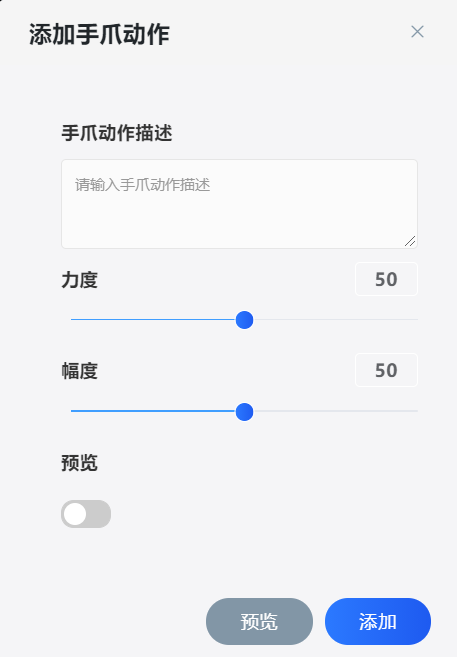
\includegraphics[height=6cm]{screen/3-12.png}
	\caption{“添加手爪动作”对话框}
	\label{fig:添加手爪动作对话框}
\end{figure}

在\nameref{fig:添加动作块弹出框}中选择\mnu{手爪},弹出\nameref{fig:添加手爪动作对话框}(如\prettyref{fig:添加手爪动作对话框})。输入手爪动作描述,设置力度和幅度。如果需要预览手爪的开闭效果,请打开\mnu{预览}开关(实时预览)或点击\btn[Info]{预览}按钮(手动预览),确认效果无误后,点击\btn{添加}。

\subsubsection{等待动作块}
在\nameref{fig:添加动作块弹出框}中选择\mnu{等待},输入等待秒数。
\subsubsection{消息提示动作块}
在\nameref{fig:添加动作块弹出框}中选择\mnu{消息提示},消息提示分为灯板提示和弹框提示。其中灯板提示可选择多种样式:
\begin{itemize}[leftmargin=4.5em]
\item[关闭] 关闭灯板显示;
\item[常亮] 灯板保持指定颜色常亮;
\item[呼吸] 灯板按照指定颜色呼吸;
\item[均分旋转] 灯板按照指定的2个或4个不同颜色平均分布旋转展示;
\item[同色旋转] 灯板按照某个颜色旋转展示;
\item[闪烁] 灯板按照某个颜色闪烁。
\end{itemize}
\subsubsection{数字I/O动作块}
在\nameref{fig:添加动作块弹出框}中选择\mnu{数字I/O},在弹出的添加对话框中,顶部标签页对应数字I/O的操作类型,数字I/O动作块支持三种类型的操作:
\begin{itemize}[leftmargin=4.5em]
\item[读取] 读取某个数字I/O端口的输入值;
\item[等待] 当执行到该动作块时,将等待某个数字I/O的值为选定的值,在未变为选定的值之前,将一直停留在该动作块;
\item[设置] 设置某个数字I/O端口的输出值。
\end{itemize}

数字I/O的端口类型,有控制箱I/O、法兰盘I/O和外置I/O(如有)三种。

\clearpage

点击\btn{添加}完成数字I/O动作块的插入。
% \begin{itemize}
% 	\item 控制箱I/O
% 	\item 法兰盘I/O
% 	\item 外置I/O
% \end{itemize}

% \info{运行任务前请确认要使用的I/O输入输出电气连接正常。}

\vfill

\info{运行任务前请确认数字I/O的输入输出电气连接正常。}

\vfill

\subsubsection{模拟I/O动作块}
在\nameref{fig:添加动作块弹出框}中选择\mnu{模拟I/O},在弹出的添加对话框中,顶部标签页对应模拟I/O的操作类型,模拟I/O动作块支持三种类型的操作:
\begin{itemize}[leftmargin=4.5em]
\item[读取] 读取某个模拟I/O端口的输入值;
\item[等待] 当执行到该动作块时,将等待某个模拟I/O的值与选定值的判断条件成立,在条件未成立之前,将一直停留在该动作块;
\item[设置] 设置某个模拟I/O端口的输出值。
\end{itemize}

模拟I/O的端口类型,仅有控制箱I/O和外置I/O(如有)两种。法兰盘暂无模拟I/O端口。

点击\btn{添加}完成模拟I/O动作块的插入。

\vfill

\info{运行任务前请确认模拟I/O的输入输出电气连接正常。}

\vfill

\clearpage

\begin{figure}[ht]
	\centering
	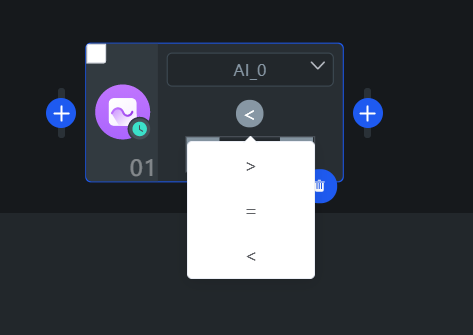
\includegraphics[height=3cm]{screen/3-13.png}
	\caption{模拟I/O判断条件}
	\label{fig:模拟IO判断条件}
\end{figure}

其中,在等待操作类型下,判断条件有:>、=、<三种,当点击某个等待模拟I/O位置块的等待条件按钮(如\prettyref{fig:模拟IO判断条件})时,进行相应的判断条件修改。

\subsubsection{负载配置动作块}
在\nameref{fig:添加动作块弹出框}中选择\mnu{负载配置},在添加负载配置对话框中输入需要修改的负载质量或质心,该功能用于在程序运行过程中动态修改负载的质量和质心。

\danger[警告]{当机器人末端安装有末端工具,且该工具具有取/放物品等功能时,需要在时间轴编辑器的对应位置插入经取/放后末端负载质量和质心对应变化的动作块,如未正常设置,可能降低机器人相应部件寿命,且可能导致碰撞检测误报。}

\danger[警告]{添加负载配置时,质量和质心的设置必须尽量与末端工具质量一致,更换或卸除末端工具时,一定要相应地修改负载参数或禁用对应的末端设备,否则有可能导致误伤。}

\subsection{工具栏}
% 时间轴编辑器的工具栏为查找、编辑、操作和执行该场景的工具区域:

\begin{figure}[ht]
	\centering
	
\includegraphics[width=\textwidth]{screen/3-14.png}
	\caption{时间轴编辑器工具栏}
	\label{fig:时间轴编辑器工具栏}
\end{figure}

\subsubsection{修改场景名称}
点击工具栏标题文字后面的\icn{image/ic_toolbar_edit.pdf}修改按钮,在弹出的场景修改对话框中修改场景名称。
\subsubsection{搜索}
点击搜索按钮,可展开动作块搜索框。

\begin{figure}[ht]
	\centering
	
\includegraphics[width=\textwidth]{screen/3-15.png}
	\caption{展开的动作块搜索框}
	\label{fig:展开的动作块搜索框}
\end{figure}

在搜索框展开状态下,点击搜索框左侧的\icn{image/all.pdf}图标,可以根据弹出框中的动作块类型来进行快速搜索。同时,也可结合文本输入框中输入的关键字来查询对应类型或全部类型下的符合该关键字的动作块。

\vfill

\subsubsection{信号量}
信号量在\LM~2.1 中暂无有效使用。

\vfill

\subsubsection{速度和加速时间}
\label{sec:速度和加速时间}
工具栏上的速度和加速时间为当前场景全局的速度和加速时间配置入口,当未使用\prettyref{sec:编辑位置}提到的单个位置动作块的速度和加速时间调整操作时,所有该场景下的位置动作块使用全局的速度和加速时间配置。

\vfill

\subsubsection{撤销/恢复}
当误删除某个动作块或者执行了错误操作时,可以点击撤销按钮\icn{image/ic_toolbar_undo.pdf}执行撤销操作;反之,如果想恢复之前被撤销的操作,可以点击恢复按钮\icn{image/ic_toolbar_redo.pdf}执行恢复操作。

\vfill

\danger[警告]{从当前编辑器页面返回或退出时,编辑器的撤销和恢复历史将被清空,再次返回当前场景编辑器时,将无法执行之前的撤销和恢复操作。}

\vfill

\clearpage

\subsubsection{删除/清空}
当编辑区选中部分动作块时,\icn{image/ic_toolbar_delete.pdf}删除/清空按钮上将展示对应选择的动作块数量,此时点击该按钮执行删除对应动作块的操作;当编辑区未选中任何动作块时,此时点击该按钮执行清空当前场景操作。

\vfill

\danger[警告]{请务必确保您已知晓执行此操作的后果并在二次确认删除或清空时,执行此操作,特别是当执行完删除或清空操作退出了当前编辑器,再次进入该场景编辑操作时,将无法还原删除或清空前的状态。}

\vfill

\subsubsection{场景循环次数}
点击时间轴编辑器工具栏右上角循环次数图标\icn{image/ic_toolbar_loops.pdf}修改任务循环次数(默认循环为1次);当次数为0时,表示执行无限循环$\infty$任务,直到机器人急停或停止。

\vfill

\subsubsection{运行场景}
\label{sec:运行场景}
运行场景有如下两种方法,可任选其一:
\begin{itemize}
	\item 点击工具栏右上角运行任务图标\icn{image/38.pdf}。
	\item 双击机器人肩部按钮,如\prettyref{fig:肩部按钮示意图}所示(肩部灯板中间有“白”标识的按钮)。
\end{itemize}

\vfill

\begin{figure}[ht]
	\centering
	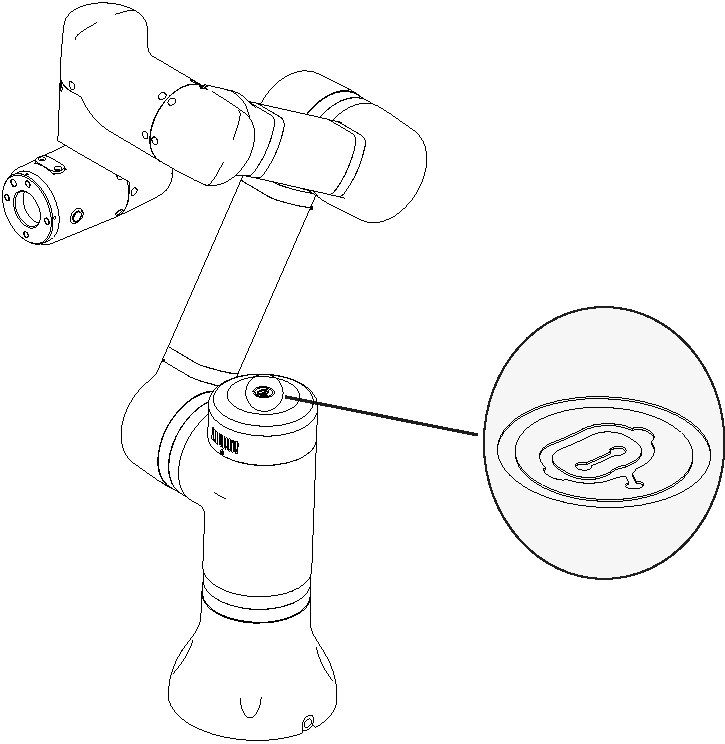
\includegraphics[height=6cm]{line_graphs/shoulder_btn.pdf}
	\caption{肩部按钮}
	\label{fig:肩部按钮示意图}
\end{figure}

\subsubsection{机器人位置安全检查}
当机器人当前位置与场景第一个待运行位置\footnote{第一个待运行位置:在时间轴编辑器中符合条件的动作块(若未选择任何动作块即表示编辑器中的所有动作块或手动选中了部分动作块即表示这部分选中的动作块)里按先后顺序查找到第一个位置类型的动作块,该动作块即第一个待运行位置,机器人控制系统会基于该动作块的位置与当前机器人的位置进行检查比对。}一致时,场景运行,不执行位置安全检查;当机器人当前位置与场景第一个待运行位置不一致时,运行场景前,会执行位置安全检查并弹出\nameref{fig:位置安全检查页}。

\begin{figure}[ht]
	\centering
	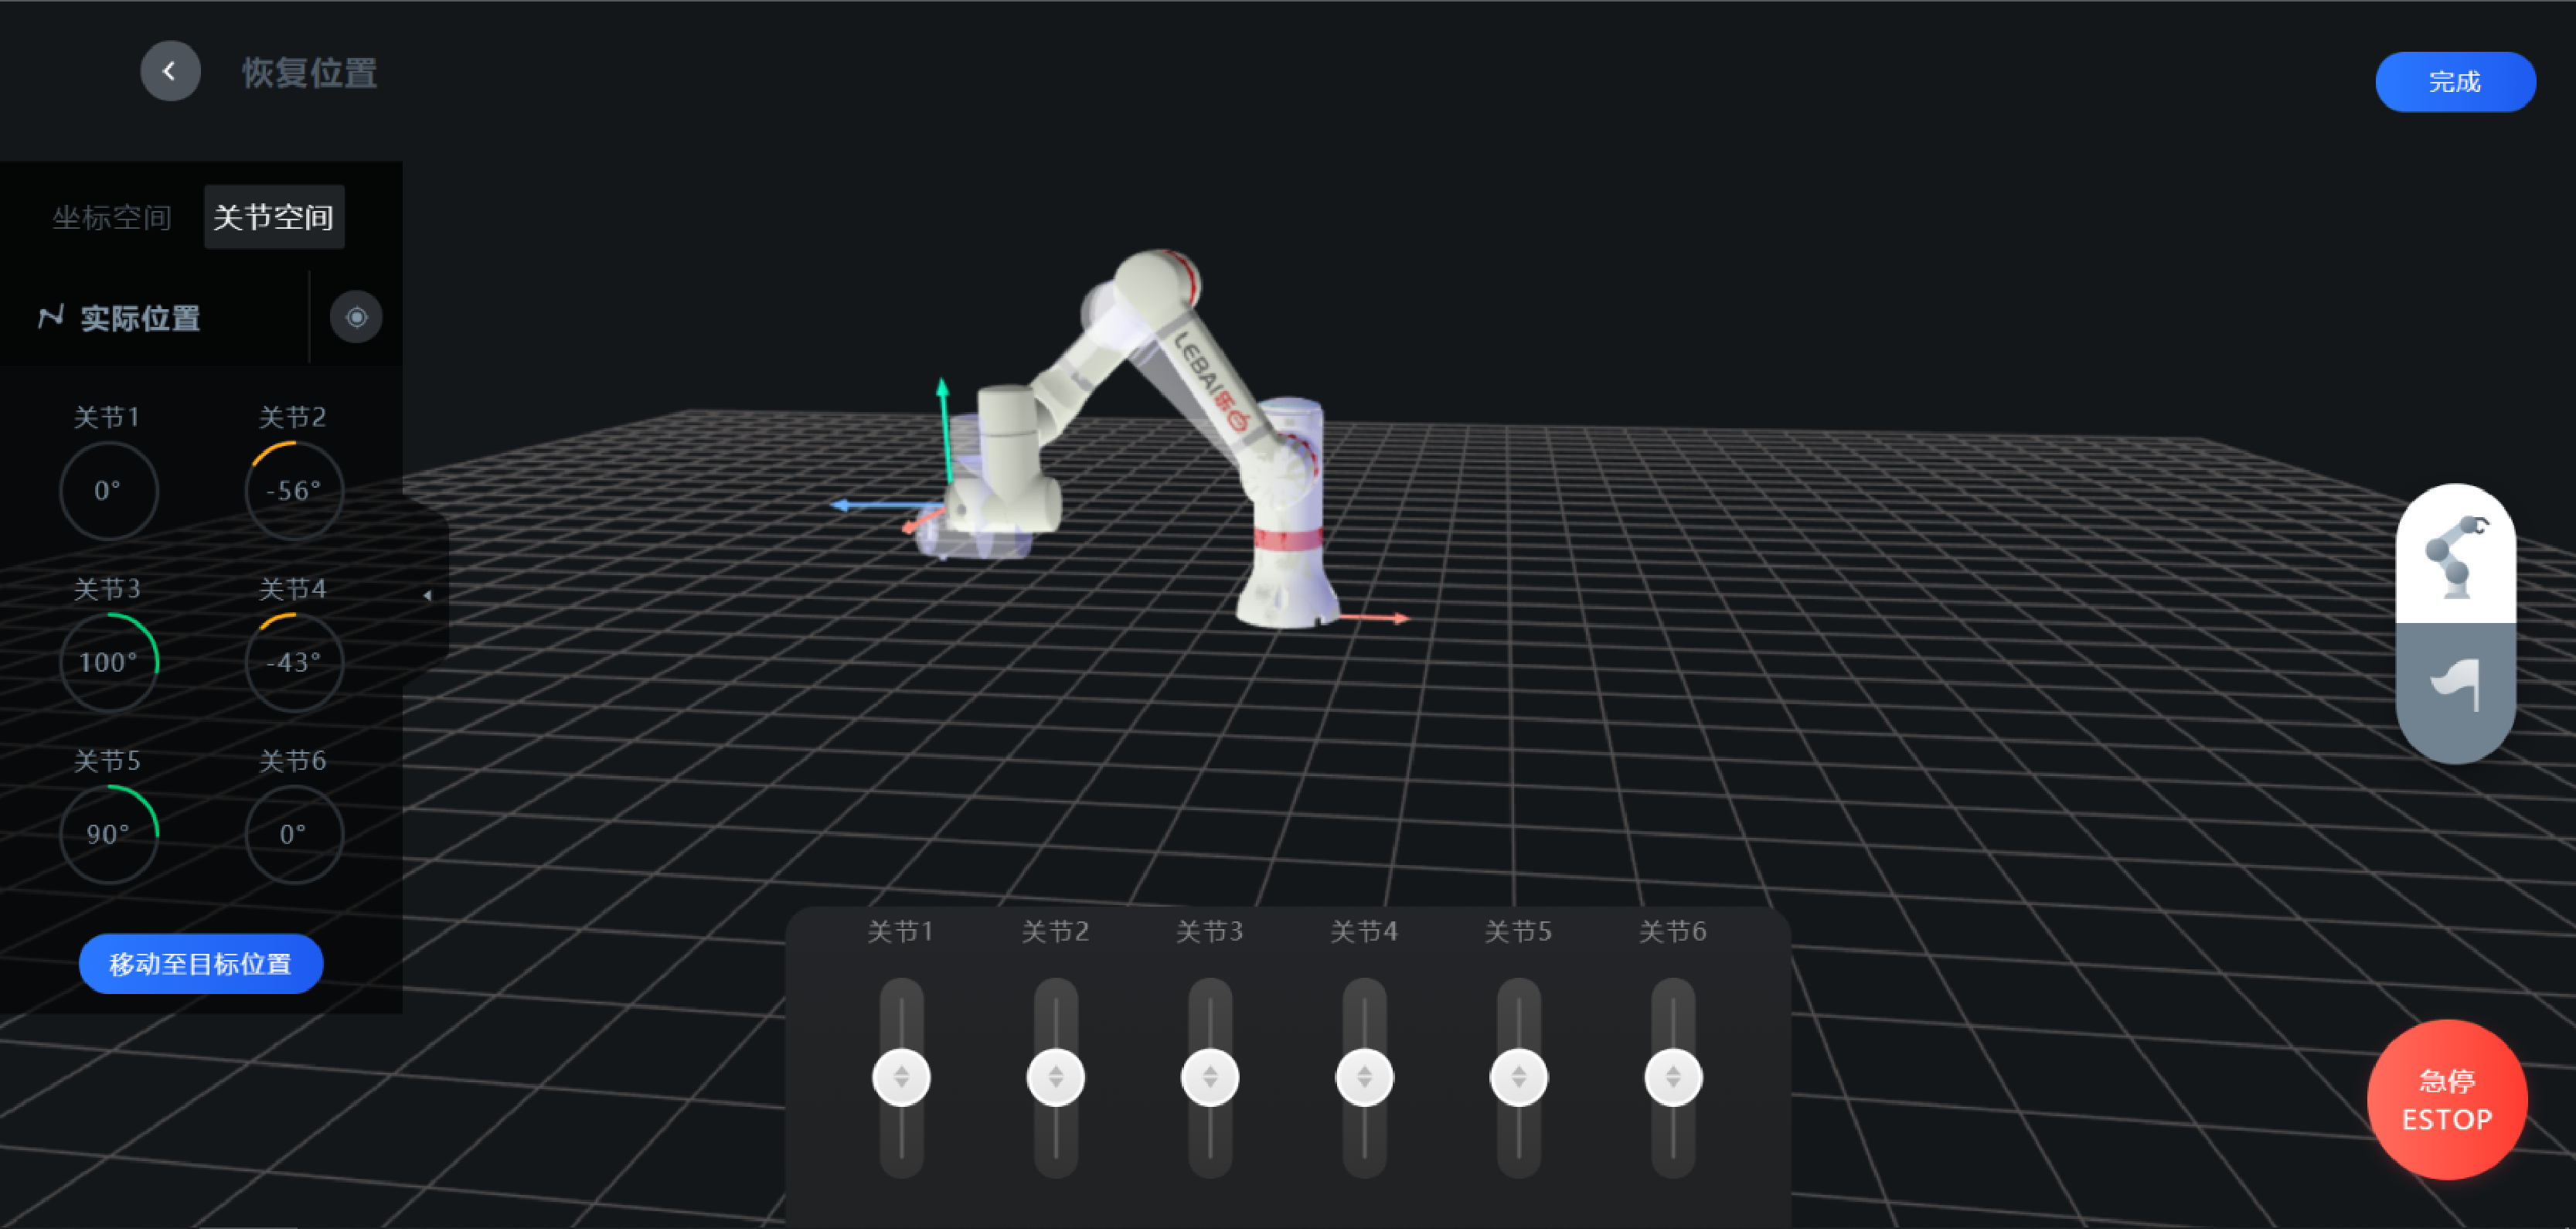
\includegraphics[width=\textwidth]{shots/position_check.pdf}
	\caption{恢复位置}
	\label{fig:位置安全检查页}
\end{figure}

在位置安全检查页可以使用如下两种操作将机器人移动到场景的第一个待运行位置:
\begin{itemize}
	\item 点击位置安全检查页\btn{移动到目标位置},等待机器人运行至场景的第一个待运行位置,运行过程中可以随时点击\btn[Danger]{停止}来停止移动。
	\item 长按末端平按钮,机器人移动到任务第一个待运行位置后,放开末端平按钮。
\end{itemize}

点击右上角\btn{完成}按钮,场景开始运行。在场景运行时,长按肩部按钮可以暂停或恢复任务。

\info{机器人当前位置与待执行场景的第一个待运行位置存在差异时,运行场景前会进行机器人位置安全检查。}

\danger[警告]{在使用末端平按钮移动到第一个待运行位置后,请与机器人保持一定安全距离,点击\btn{完成}按钮去运行场景,否则可能会造成误伤。}

\subsection{操作技巧}
\subsubsection{快速搜索动作块}
右键单击某个动作块,在弹出的右键菜单中选择\mnu{查找相似块},可快速搜索出相同动作块类型且包含当前选中的动作块标题作为关键字的动作块。
\subsubsection{批量编辑动作块}
% \def\ttt{通过搜索框或快速搜索动作块等操作或者手动选中}
\def\ttt{通过选中}
\ttt 2个或以上的同类型或子类型(如果该类型动作块存在子类型的话)相同的动作块。

\begin{figure}[htb]
	\centering
	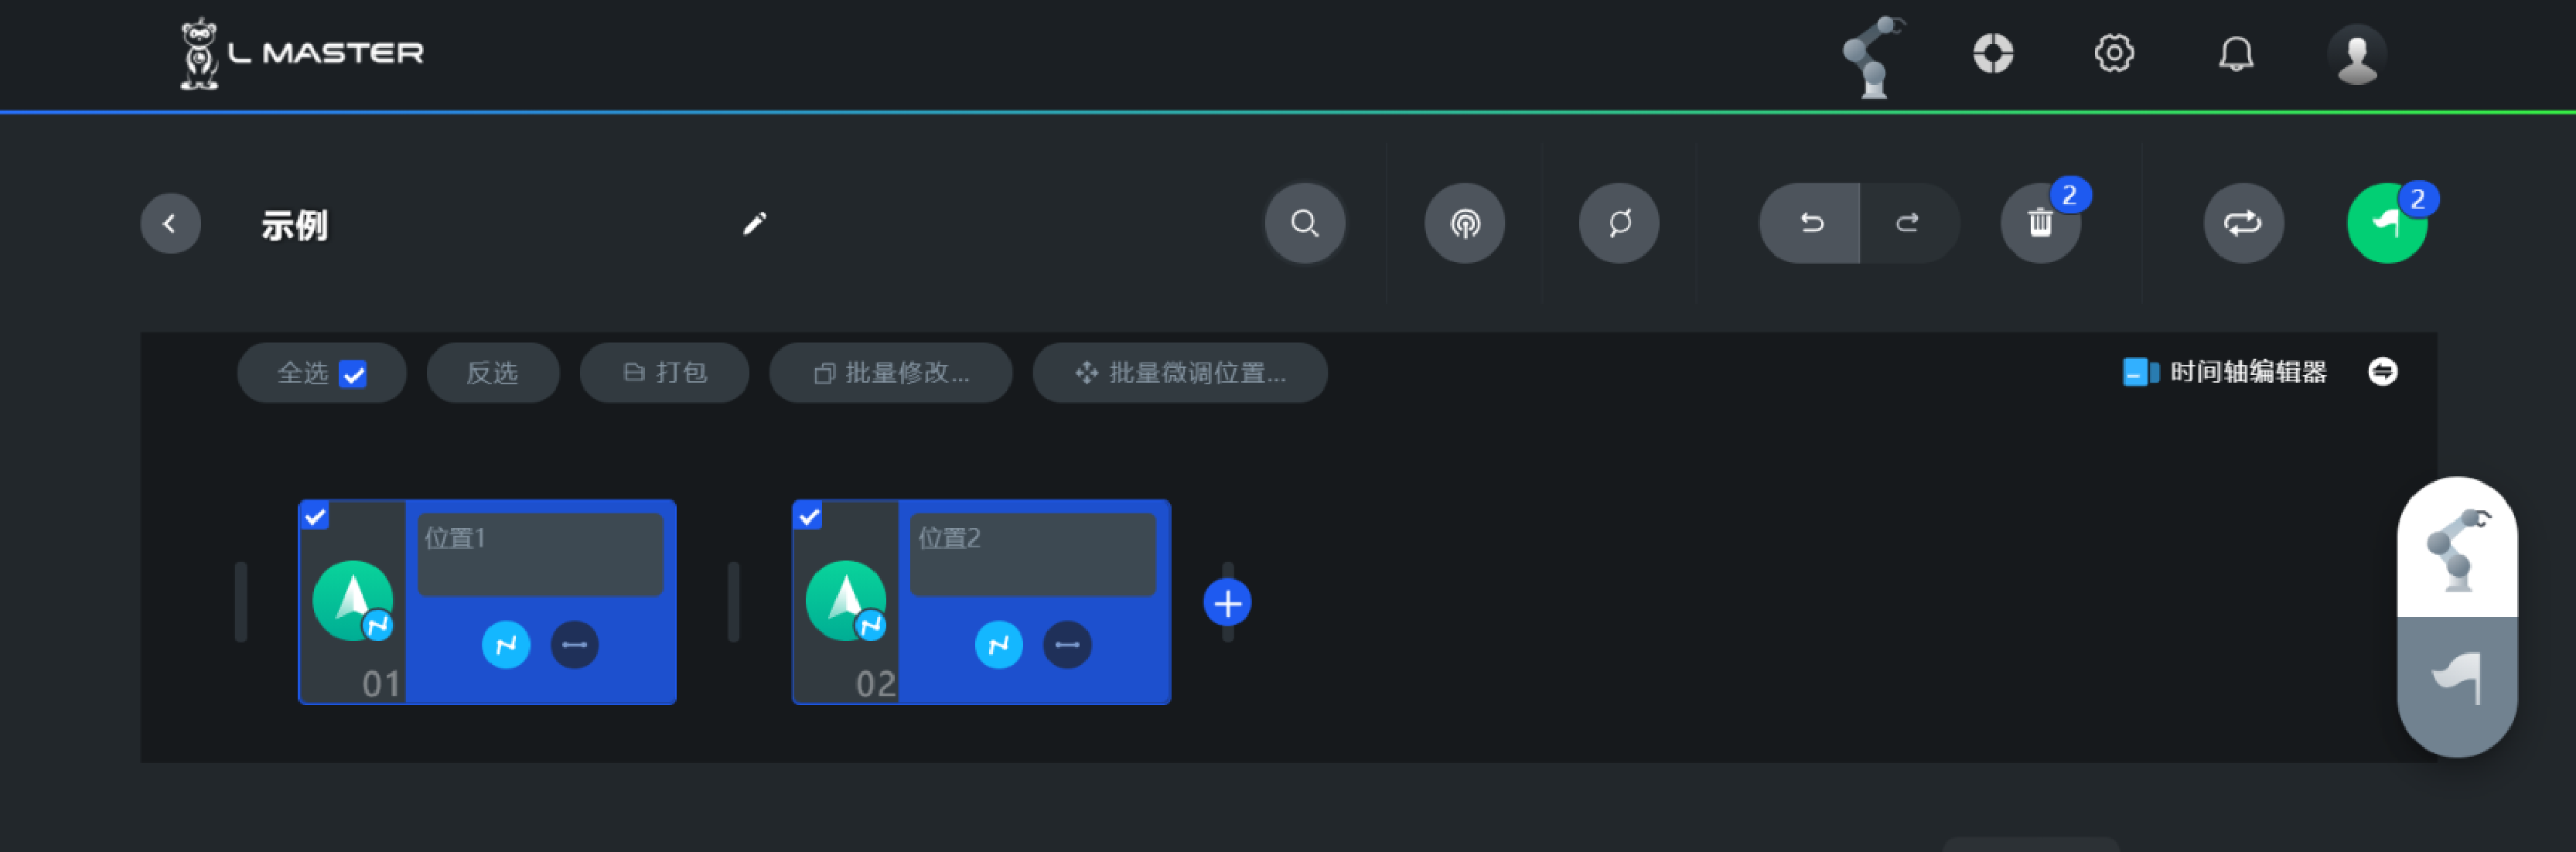
\includegraphics[width=\textwidth]{shots/batch_edit.pdf}
	\caption{批量编辑动作块}
	\label{fig:批量编辑动作块}
\end{figure}

点击场景编辑器功能区的\btn[Info]{批量修改…}按钮,或者用鼠标右键点击动作块选择\mnu{批量修改…},可对动作块以下内容进行批量编辑。

\begin{itemize}[leftmargin=7.5em]
\item [位置动作块] 统一修改位置名称、切换关节空间的运动(movej)和笛卡尔空间的直线运动(movel),速度及加速时间以及启用和禁用平滑功能,且批量修改确认后每个位置块的位置数据将应用机器人当前状态下的位置数据。
\item [手爪动作块] 可以修改手爪动作描述、力度以及幅度。
\item [等待动作块] 等待秒数以及等待的目的/作用描述。
\item [消息提示动作块] 灯板提示和弹窗提示是不同子类型的动作块,不同子类型的动作块不可批量修改。
\item [数字I/O动作块] 读取、等待或设置的批量修改。
\item [模拟I/O动作块] 读取、等待或设置的批量修改。
\item [负载配置动作块] 支持同子类型的负载质量或质心的批量修改。
\end{itemize}

点击对话框右下角的\btn{修改}按钮可应用批量编辑操作,点击右上角的\kbd{$\times$}按钮可取消批量编辑操作。

\info{动作块批量编辑,动作块类型和子类型(如果该类型动作块存在子类型的话)必须一致。}

\clearpage

\subsubsection{批量微调位置块}
选中2个或以上的位置动作块,点击时间轴编辑器功能区的\btn[Info]{批量微调位置…},或者将光标放在选中的位置动作块上使当前位置动作块处于焦点状态,在右键单击弹出的右键菜单中,选择 \mnu{批量微调位置…},进入\mnu{调整位置}页面\footnote{详见\prettyref{sec:微调}。}。

\begin{figure}[hb]
	\centering
	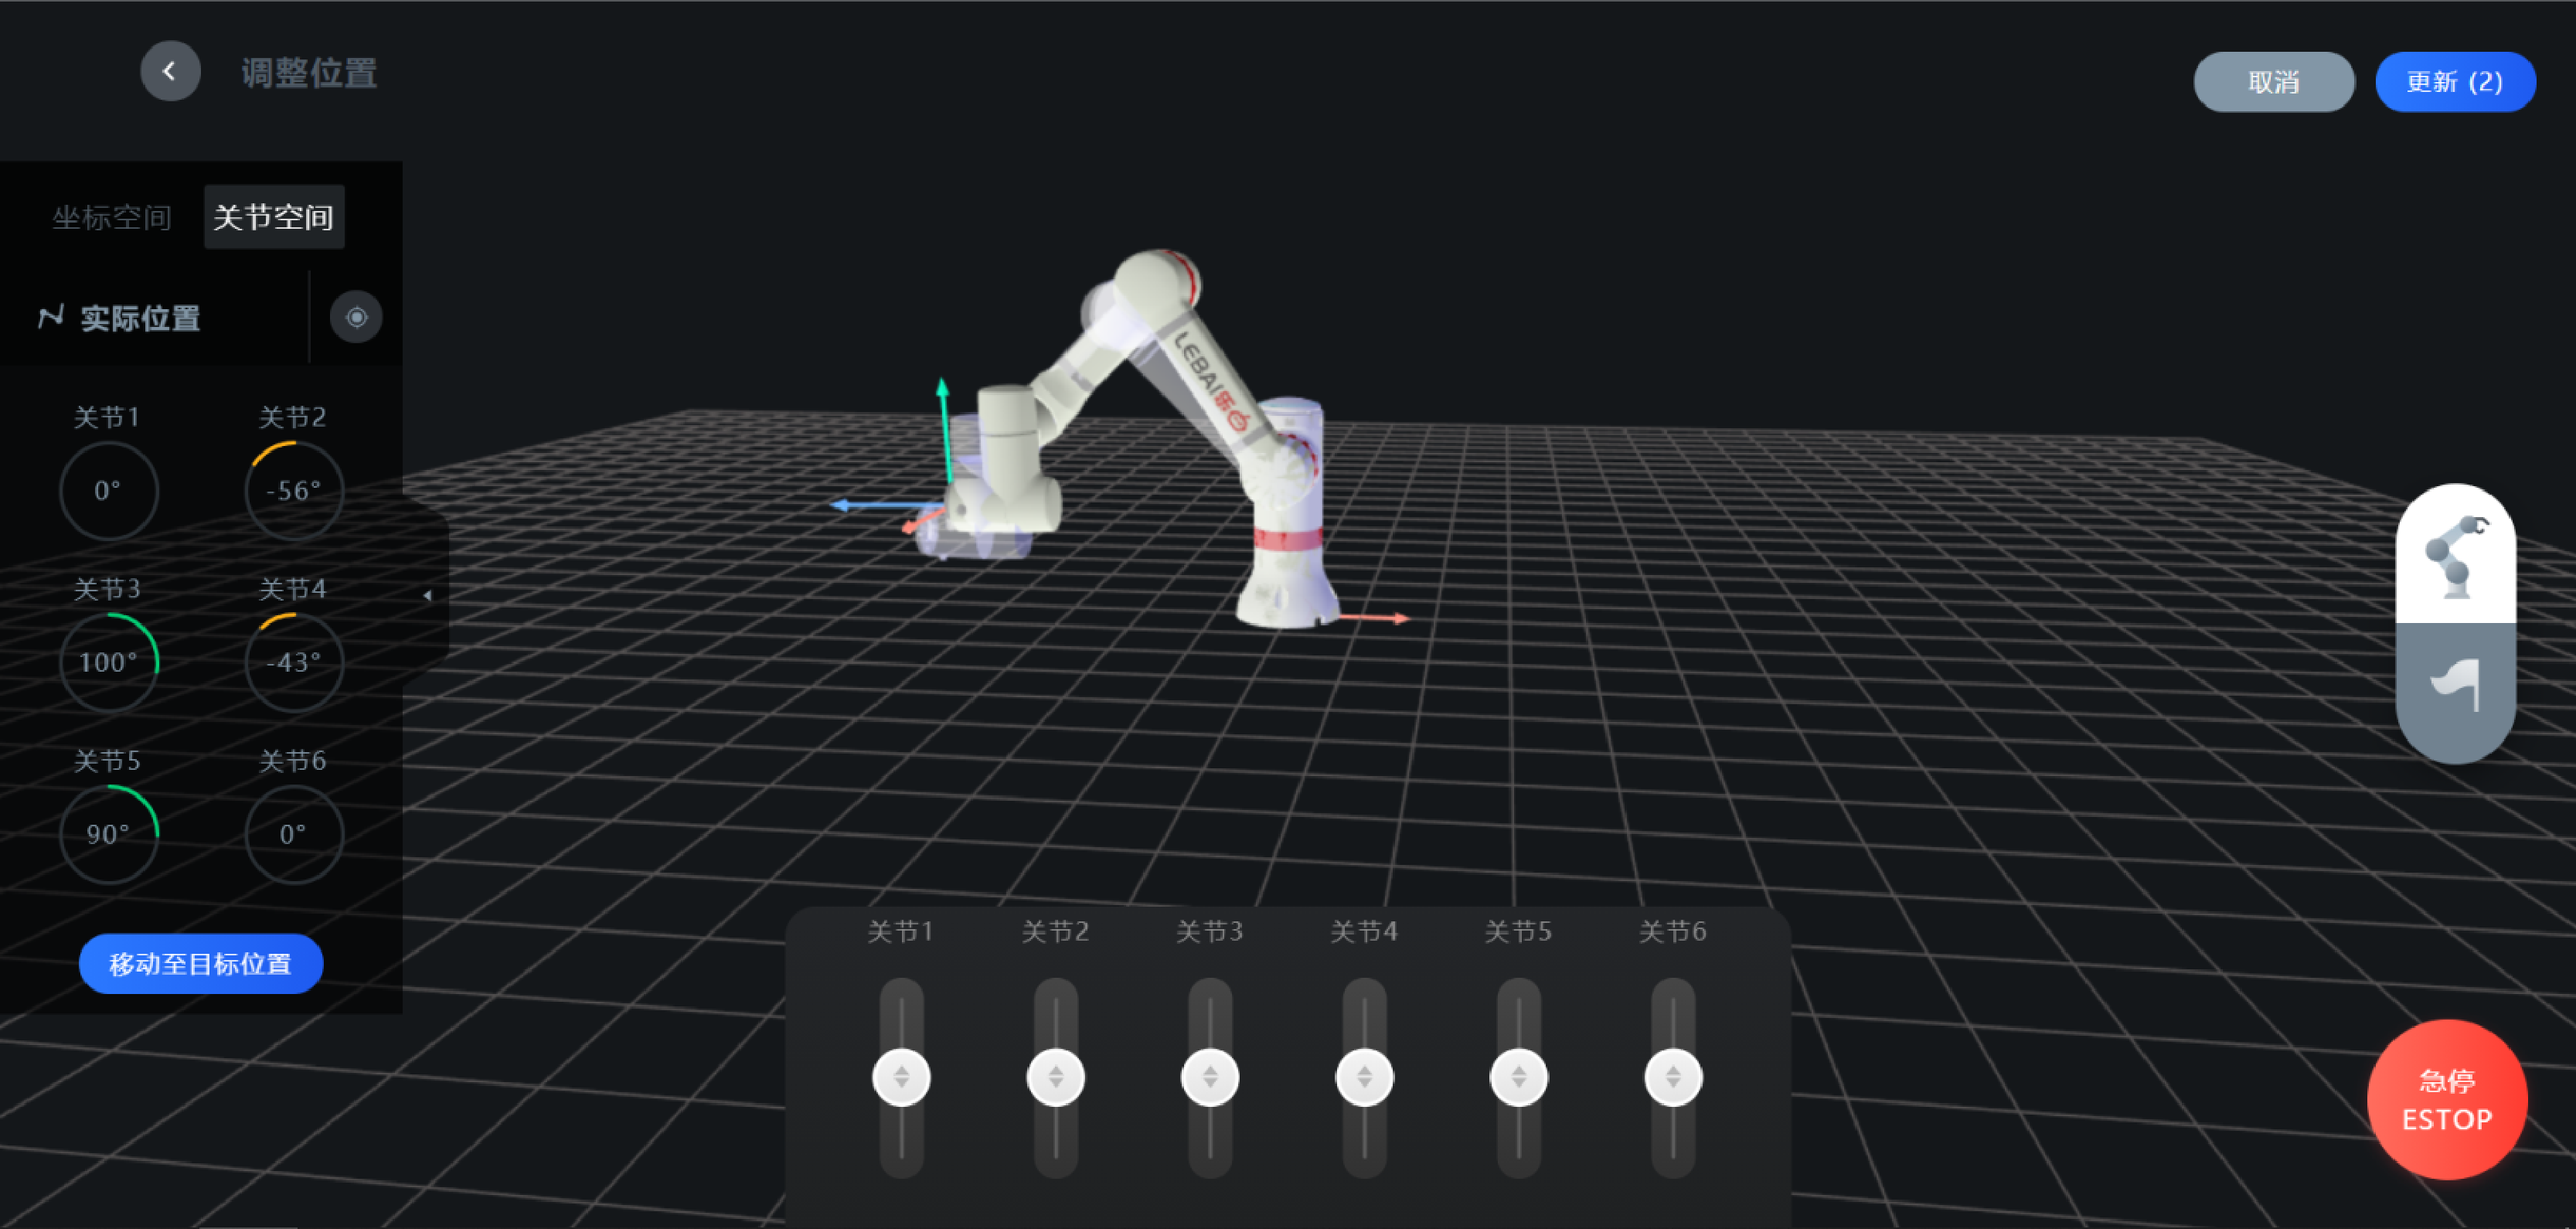
\includegraphics[width=\textwidth]{shots/batch_adjust_positions.pdf}
	\caption{批量微调位置块}
	\label{fig:批量微调位置块}
\end{figure}

微调移动至目标位置后,点击页面右上角的\btn{更新}按钮,完成批量微调;点击\btn[Info]{取消}可放弃批量微调操作。其中,\btn{更新}按钮右侧数字表示当前选中的位置块总数。

\clearpage

\subsection{导出场景}
\label{sec:导出场景}
在场景列表页面选择需要保存的场景,鼠标移动到场景卡片右上角\icn{image/vdots.pdf}按钮,弹出场景菜单,选择\mnu{导出},在弹出的保存对话框选择场景文件的保存位置(场景文件后缀名为 \verb|lbd|)。

\begin{figure}[htb!]
	\centering
	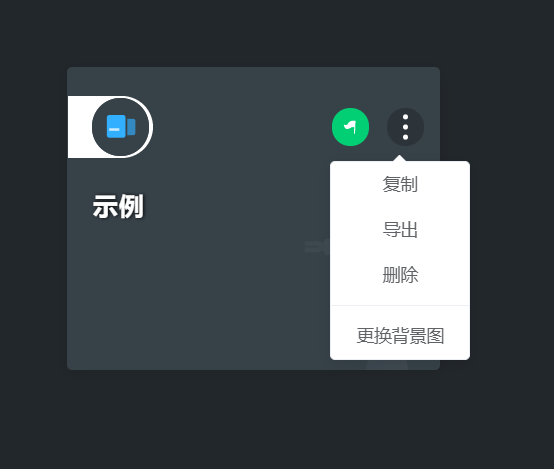
\includegraphics[height=3cm]{screen/3-19.png}
	\caption{导出场景}
	\label{fig:导出场景}
\end{figure}

\subsection{导入场景}
\label{sec:导入场景}
如\prettyref{fig:导入场景},在\mnu{场景列表}的工具栏中点击\icn{image/icon_import.pdf}导入场景,打开之前导出的场景文件,导入完成后会自动进入该场景。

\begin{figure}[htb!]
	\centering
	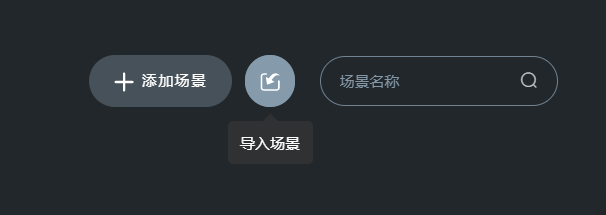
\includegraphics[height=1.8cm]{screen/3-20.png}
	\caption{导入场景}
	\label{fig:导入场景}
\end{figure}

\clearpage

\section{控制}
控制模块主要分为:
\begin{itemize}
\item 虚拟控制
\item 位置库
\item I/O控制
\item 手爪控制
\item 硬件按钮
\item 灯板控制
\end{itemize}

\subsection{虚拟控制}
通过虚拟控制可以调整机器人当前位置与姿态,具体操作方式参考\prettyref{sec:微调}中的微调功能介绍。

\begin{figure}[ht]
	\centering
	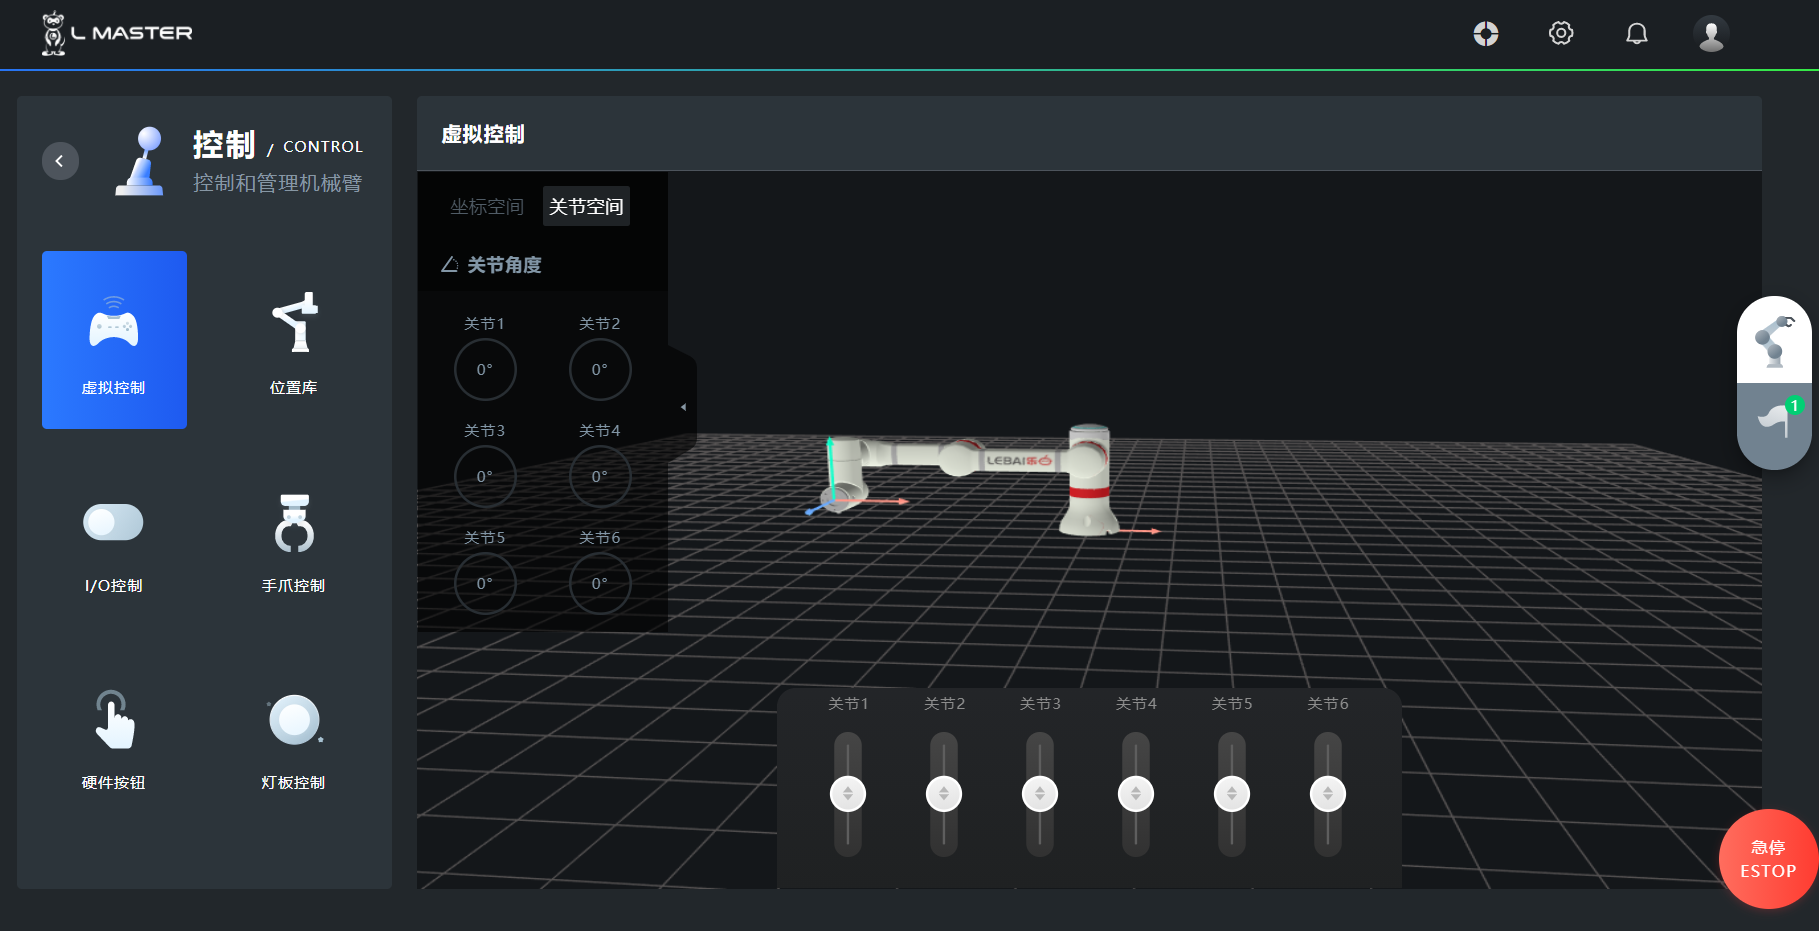
\includegraphics[width=\textwidth]{screen/3-21.png}
	\caption{虚拟控制}
	\label{fig:虚拟控制示意图}
\end{figure}

\subsection{硬件按钮}
\label{sec:硬件按钮}

\begin{figure}[ht]
	\centering
	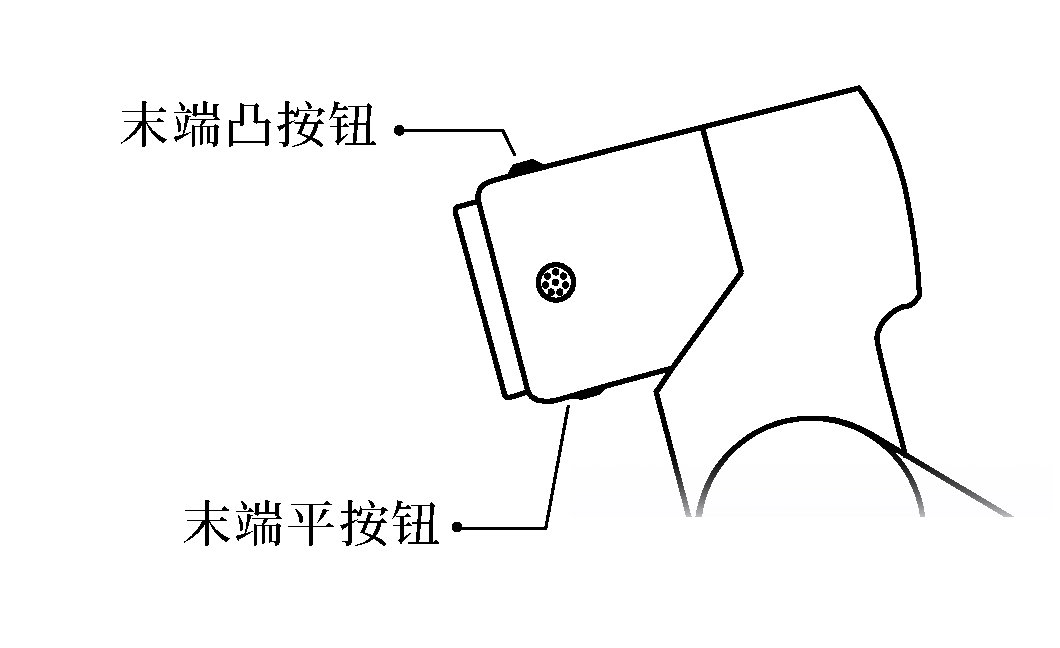
\includegraphics[height=3cm]{line_graphs/flange_buttons.pdf}
	\caption{末端按钮示意图}
	\label{fig:末端按钮示意图}
\end{figure}

\begin{enumerate}[label=(\arabic*)]
	\item 末端平按钮
	\begin{itemize}
		\item[单击] 时间轴编辑焦点往后移动一个动作块;
		\item[双击] 时间轴编辑焦点往前移动一个动作块;
		\item[长按] 当前如果处于位置动作块刷新位置弹框(点击位置块的微调按钮进入)或者位置库应用位置弹框时,则移动到对应的目标位置;
		\item[释放] 当长按进入移动到目标位置操作时,释放将停止当前移动。
	\end{itemize}

	\item 末端凸按钮
	\begin{itemize}
		\item[长按] 进入示教模式;
		\item[释放] 退出示教模式;
		\item[双击] 在编辑器中添加一个位置动作块/代码;
		\item[单击] 当前动作块为位置动作块的前提下 ,如果当前位置动作块未进入微调位置对话框,单击该按钮进入微调当前位置对话框; 如果当前已进入微调位置对话框,单击该按钮则表示更新当前动作块保存的位置数据。
	\end{itemize}

	\item 肩部按钮
	\begin{itemize}
		\item[长按] 切换队列暂停/恢复操作,即\mnu{运行中}时暂停,\mnu{暂停}时恢复;
		\item[单击] 场景编辑器有弹框时或者其他界面,等价于点击取消操作(按钮,对话框等);
		\item[双击] 当前在场景编辑器界面且无其他弹框,则切换运行/停止操作 ;场景编辑器有弹框时或者其他界面,等价于点击确认操作(按钮、对话框等)。
	\end{itemize}

	\item 按钮组合操作
	\begin{itemize}
		\item 启动/停止机器人:长按末端平按钮,同时长按肩部按钮,可以切换启动和停止机器人的操作。

	\end{itemize}
\end{enumerate}
		\info{启动/停止机器人的按钮组合操作仅在当前机器人未急停或未断电时有效。}

\section{设备}
\subsection{末端设备}
\label{sec:末端设备}
如果需要在机器人末端添加末端工具(如:手爪),点击\mnu{设备},在末端设备点击\btn{添加},设置相应的辅助工具的质量和质心,点击\mnu{启用}。如果需要卸除末端工具,点击\mnu{禁用}。

\danger[警告]{\begin{itemize}
	\item 添加末端设备时,末端设备的质量和质心的设置须与末端工具质量和质心尽可能一致。
	\item 更换或卸下末端工具时,一定要相应地修改末端设备的质量和质心或关闭对应末端设备,否则有可能导致误伤。
\end{itemize}}

\section{设置}
\subsection{TCP设置}
\label{sec:TCP设置}
TCP意为机器人工具中心点(Tool Center Point)。TCP设置页用于设置机器人末端TCP位置和姿态的偏移量/转换量。默认不设置TCP,当机器人装载末端工具时可以根据场景应用需要选择性添加TCP设置。

TCP可以通过示教的方式进行添加。点击\btn{添加}按钮菜单的\mnu{示教添加},打开\nameref{fig:示教添加TCP设置},如\prettyref{fig:示教添加TCP设置}。此时可点击示教图标,拖动示教机器人,使得机器人末端工具在接触同一控制点(即保持末端工具始终接触同一个位置)的情况下,以四个不同姿态逐一确认四个关键点,机器人根据末端法兰不同的位置和方向,可自动识别TCP位置信息。姿态信息需要手动填写,暂不支持示教添加。

\begin{figure}[htb]
	\centering
	\begin{minipage}[t]{0.48\linewidth}
		\centering
		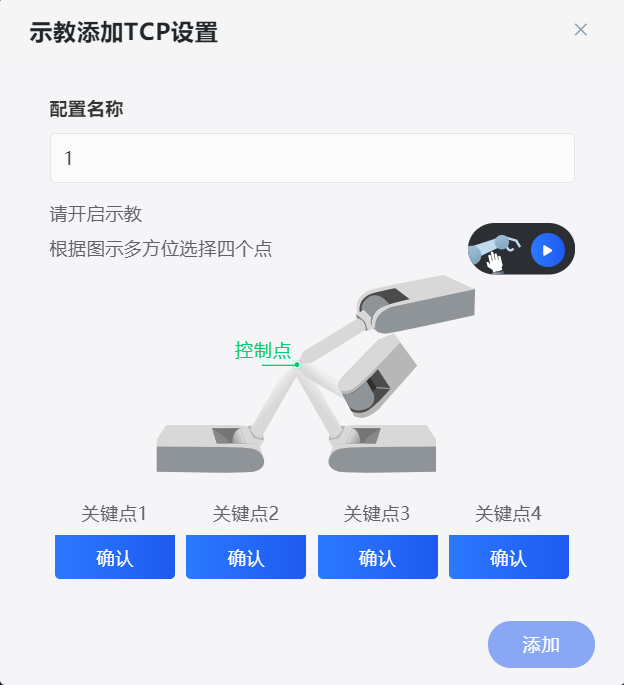
\includegraphics[width=\linewidth]{screen/3-24.png}
		\caption{示教添加TCP设置}
		\label{fig:示教添加TCP设置}
	\end{minipage}
	\hfill
	\begin{minipage}[t]{0.48\linewidth}
		\centering
		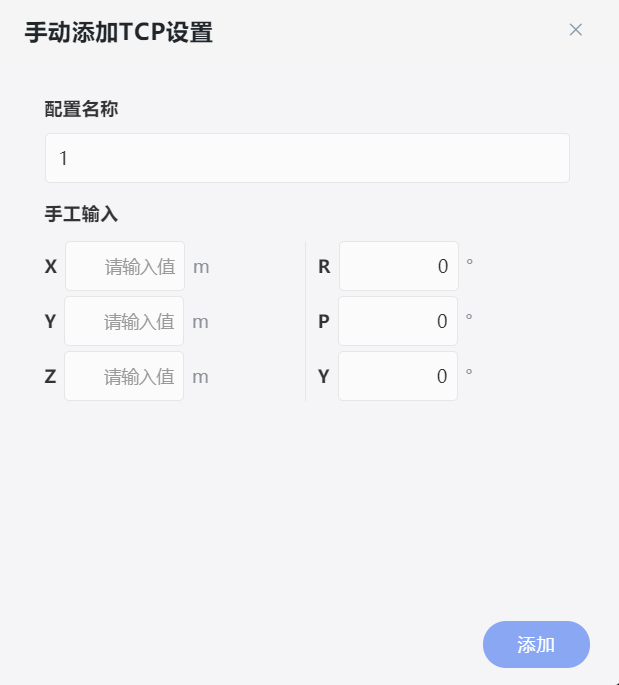
\includegraphics[width=\linewidth]{screen/3-25.png}
		\caption{编辑TCP设置}
		\label{fig:编辑TCP设置}
	\end{minipage}
\end{figure}

用户还可以通过\mnu{手动添加}或者\btn[Card]{编辑},进入\nameref{fig:编辑TCP设置},如\prettyref{fig:编辑TCP设置},手动设置末端工具的位置和姿态。

\vfill

\subsection{安全设置}
\subsubsection{碰撞检测}
机器人碰撞检测在安装引导页开启后默认状态为\mnu{急停}。机器人在运行任务过程中,检测到外部阻力的碰撞后的动作分为\mnu{暂停}和\mnu{急停}两种,同时用户可以自行调节检测的灵敏度。

\begin{figure}[htb]
	\centering
	\subfigure[急停]{\begin{minipage}[t]{0.48\linewidth}
		\centering
		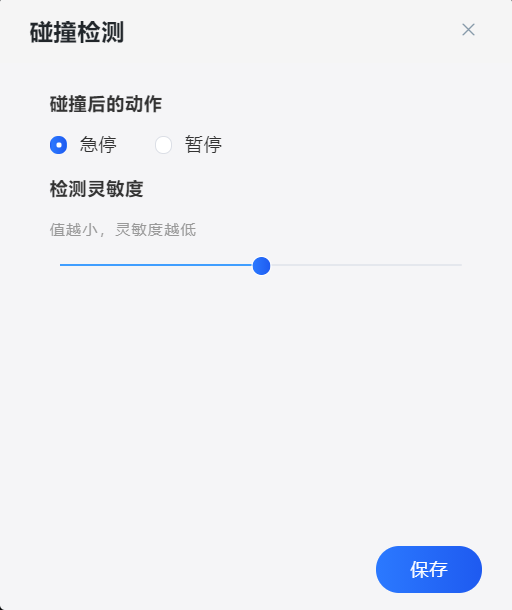
\includegraphics[width=\linewidth]{screen/3-26-1.png}
	\end{minipage}}
	\hfill
	\subfigure[暂停]{\begin{minipage}[t]{0.48\linewidth}
		\centering
		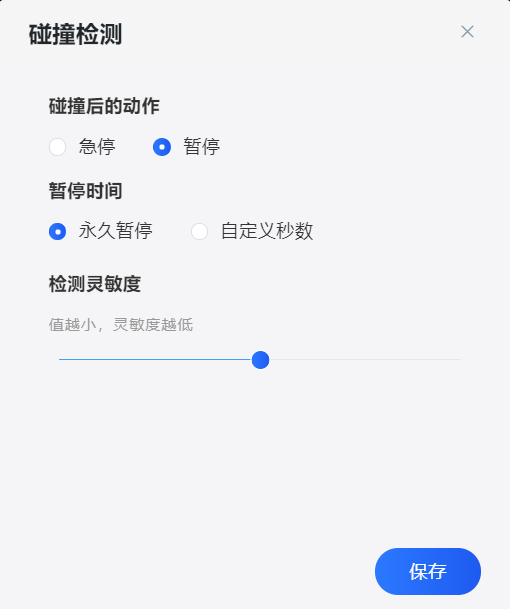
\includegraphics[width=\linewidth]{screen/3-26-2.png}
	\end{minipage}}
	\caption{碰撞检测}
	\label{fig:碰撞检测设置}
\end{figure}

碰撞后的动作:
\begin{itemize}
	\item[急停] 需要重新启动机器人,示教至安全位置后才能继续操作。
	\item[暂停] 若选择自定义秒数,到达指定暂停时间时,任务会自动恢复运行;若选择永久暂停,需要在首页任务历史列表栏点击恢复任务按钮\icn{image/39.pdf}。
\end{itemize}

\subsubsection{运行安全}
\label{sec:运行安全}
在运行安全中,可以查看和调整如下运行时的参数:
\begin{itemize}
	\item 每个关节的最大角度和最小角度
	% \item 在关节空间运行时的最大速度和最大加速度限制
	% \item 在坐标空间运行时的最大速度和最大加速度限制
	\item 关节空间运行配置
	\item 坐标空间运行配置
\end{itemize}

% 其中,关节空间运行时的最大速度和最大加速度限制应用于场景编辑在时间轴编辑器模式下,使用滑杆调整速度和加速时间(加速度)时的最大值,控制系统限制关节空间相关移动(movej)的速度和加速度的最大值以及全局限定每个关节运行时的最大速度限制时有效。当任意一个关节运行时的速度超过最大速度限制时,机器人会自动急停。

% 坐标空间运行时的最大速度和最大加速度限制应用于场景编辑器在时间轴编辑器下,使用滑杆调整速度加速时间(加速度)时的最大值以及控制系统限制坐标空间相关移动(movel, movec)的速度和加速度的最大值。

\begin{figure}[htb!]
	\centering
	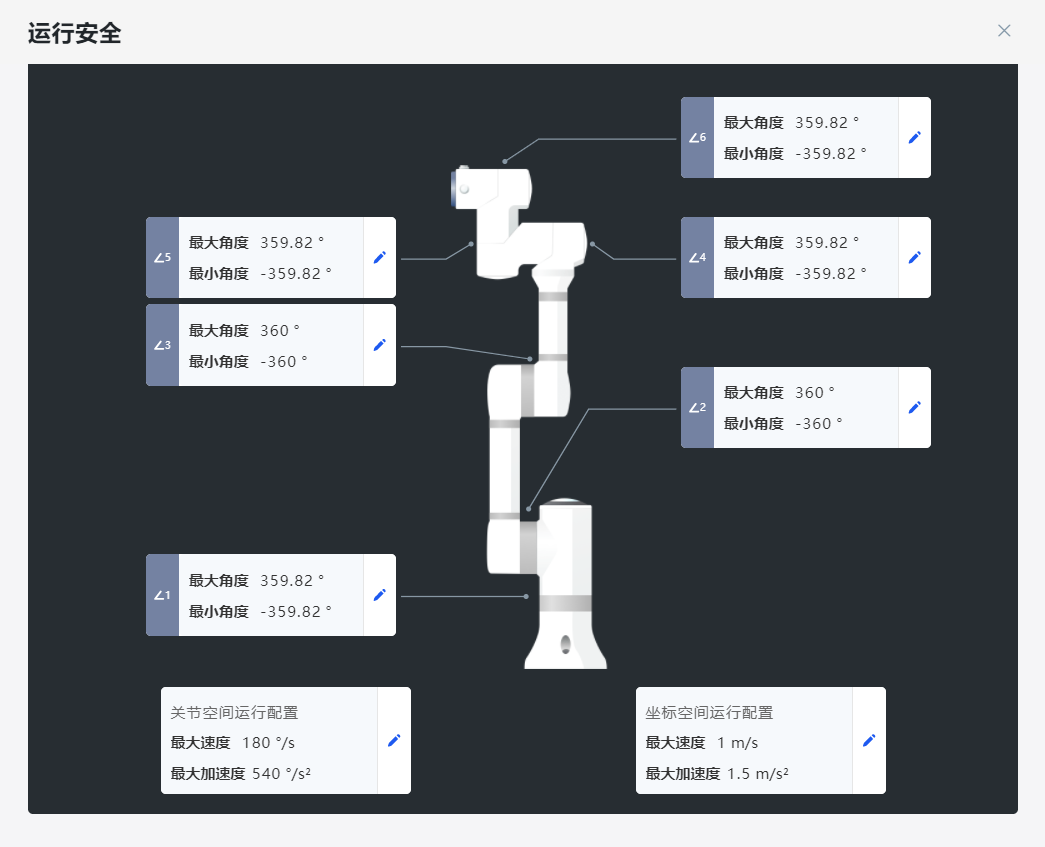
\includegraphics[height=7.5cm]{screen/3-27.png}
	\caption{运行安全设置}
	\label{fig:运行安全设置}
\end{figure}

\info{关节的最小角度和最大角度理论上可以设置为任意值。出厂时预置有默认值限制,建议使用默认值。如需调整,为了编程和调试方便,用户可以设置为$-360\sim 360^\circ$。}

\info{修改关节空间运行配置会影响机器人的速度限制。当任意一个关节运行时的速度超过最大速度限制时,机器人会自动急停。}

\danger{修改关节空间运行配置及修改坐标空间运行配置,会等比例影响场景编辑器中位置动作块的速度。}

% \danger[警告]{非专业用户在不确定修改后的风险情况下,不可随意更改。}

% \clearpage

\subsection{操作模式}
操作模式分为如下两种,可根据实际情况选择:
\paragraph{新手模式}
新手模式使用低门槛时间轴编辑器。在新手模式下,专家模式的部分功能将被隐藏,以减少复杂和高级功能带来的困扰。
\paragraph{专家模式}
% 专家模式使用专业代码编辑器。
在专家模式下:
\begin{itemize}
\item 可支持切换编辑器类型为代码编辑器(代码编辑器使用Lua语言进行编辑)。
\item 支持将时间轴编辑器版本的场景转换成Lua代码 。
\item 支持时间轴编辑器模式下关闭位置安全检查。
\item 支持安装设置可自定义任意安装方式的配置。
\end{itemize}

\info{请务必确保您已足够了解该操作的危险性后再关闭位置安全检查。}

\vfill

操作模式的切换:
\begin{itemize}
	\item 在\mnu{设置}页面的\mnu{操作模式}中切换并保存。
	\item 场景编辑右上角的切换图标,切换并保存。
\end{itemize}

\vfill

\clearpage

\subsection{系统更新}

进入\mnu{设置}的\mnu{系统更新}页后,如果当前系统已是最新版本,画面中心图标显示蓝色,如\prettyref{fig:系统更新}。点击\btn{检查系统},画面中心圆形图案显示\mnu{正在检查更新}。

\begin{figure}[htb]
	\centering
	\subfigure[已是最新版本]{\begin{minipage}[t]{0.3\linewidth}
		\centering
		
\includegraphics[width=\linewidth]{screen/3-28.png}
	\end{minipage}}
	\qquad
	\subfigure[检测到更新]{\begin{minipage}[t]{0.3\linewidth}
		\centering
		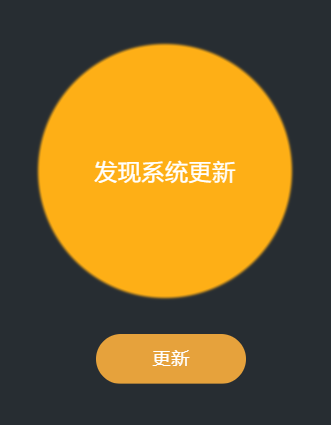
\includegraphics[width=\linewidth]{screen/3-29.png}
	\end{minipage}}
	\caption{系统更新}
	\label{fig:系统更新}
\end{figure}

当检测到系统版本有更新时,画面中心图标显示橙色,并提示“发现系统更新及最新版本号”,点击下方\btn[Warning]{更新},系统自动更新至最新版本。

\info{\begin{itemize}
	\item 请确认机器人状态为\mnu{停止},再进行系统更新。
	\item 系统更新中,不可进行其他操作,否则可能导致机器人系统损坏等严重后果。
\end{itemize}}
